\documentclass[11pt]{article}

\usepackage{macros}

\title{Course Notes for EE227C (Spring 2018):\\
 Convex Optimization and Approximation }
\author{Instructor: Moritz Hardt\\
{\small Email: \tt hardt+ee227c@berkeley.edu}\\ ~\\
Graduate Instructor: Max Simchowitz\\
{\small Email: \tt msimchow+ee227c@berkeley.edu}\\ ~\\
}


\begin{document}

\maketitle

\begin{abstract}
This course explores some theory and algorithms for nonlinear optimization. We
will focus on problems that arise in machine learning and modern data analysis,
paying attention to concerns about complexity, robustness, and implementation in
these domains. We will also see how tools from convex optimization can help
tackle non-convex optimization problems common in practice.

Code examples are available at:

\begin{center}
{\Large \url{https://ee227c.github.io/}.}
\end{center}

Below are the course notes for EE227C (Spring 2018): Convex Optimization and
Approximation, taught at UC Berkeley. 
\end{abstract}


\pagebreak

\setcounter{tocdepth}{2}
\tableofcontents

\pagebreak

\part{Gradient methods}
\section{Lecture 1: Convexity}
\sectionlabel{convexity}

This lecture provides the most important facts about convex sets and convex
functions that we'll heavily make use of. These are often simple consequences of
Taylor's theorem.

\subsection{Convex sets}

\begin{definition}[Convex set]
A set $K\subseteq\R^n$ is \emph{convex} if it the line segment between any two points in~$K$ is also contained in~$K.$ Formally, for all $x,y\in K$ and all scalars $\gamma\in[0,1]$ we have $\gamma x+(1-\gamma)y\in K.$
\end{definition}

\begin{theorem}[Separation Theorem]
\theoremlabel{separation}
Let $C, K\subseteq\R^n$ be convex sets with empty intersection $C\cap K=\emptyset.$ Then there exists a point $a\in\R^n$ and a number $b\in\R$ such that
\begin{enumerate}
\item for all $x\in C,$ we have $\langle a, x\rangle \ge b.$
\item for all $x\in K,$ we have $\langle a, x\rangle \le b.$
\end{enumerate}
If $C$ and $K$ are closed and at least one of them is bounded, then we can replace the inequalities by strict inequalities.
\end{theorem}
The case we're most concerned with is when both sets are compact (i.e., closed and bounded). We highlight its proof here.
\begin{proof}[Proof of \theoremref{separation} for compact sets.]
In this case, the Cartesian product $C\times K$ is also compact. Therefore, the
distance function $\|x-y\|$ attains its minimum over $C\times K.$ Taking $p, q$
to be two points that achieve the minimum. A separating hyperplane is given by
the hyperplane perpendicular to $q-p$ that passes through the midpoint between
$p$ and $q.$ That is, $a=q-p$ and $b=(\langle a, q\rangle - \langle a,
p\rangle)/2.$ For the sake of contradiction, suppose there is a point~$r$ on
this hyperplane contained in one of the two sets, say,~$C.$ Then the line
segment from $p$ to $r$ is also contained in~$C$ by convexity. We can then find
a point along the line segment that is close to $q$ than $p$ is, thus
contradicting our assumption.
\end{proof}

\subsubsection{Notable convex sets}
\begin{itemize}
\item Linear spaces $\{x\in\R^n\mid Ax=0\}$ and halfspaces $\{x\in\R^n \mid \langle a, x\rangle \ge 0 \}$
\item Affine transformations of convex sets. If $K\subseteq\R^n$ is convex, so is $\{Ax+b\mid x\in K\}$ for any $A\in\R^{m\times n}$ and $b\in\R^m.$
In particular, affine subspaces and affine halfspaces are convex.
\item Intersections of convex sets. In fact, every convex set is equivalent to the intersection of all affine halfspaces that contain it (a consequence of the separating hyperplane theorem).
\item The cone of positive semidefinite matrices, denotes, $S^n_+ = \{ A\in\R^{n\times n}\mid A\succeq 0\}.$ Here we write $A\succeq 0$ to indicate that $x^\trans A x\ge 0$ for all $x\in\R^n.$ The fact that $S^n_+$ is convex can be verified directly from the definition, but it also follows from what we already knew. 
Indeed, denoting by $S_n=\{A\in\R^{n\times n}\mid A^\trans = A\}$ the set of all $n\times n$ symmetric matrices, we can write $S^n_+$ as an (infinite) intersection of halfspaces $S^n_+=\bigcap_{x\in\R^n\backslash\{0\}} \{ A\in S_n\mid x^\trans A x\ge 0\}.$
\item See Boyd-Vandenberghe for lots of other examples.
\end{itemize}

\subsection{Convex functions}

\begin{definition}[Convex function]
A function $f\colon\domain\to\R$ is \emph{convex} if for all $x,y\in\domain$ and all scalars $\gamma\in[0,1]$ we have $f(\gamma x+(1-\gamma)y)\le \gamma f(x)+(1-\gamma)f(y).$
\end{definition}

Jensen (1905) showed that for continuous functions, convexity follows from the ``midpoint'' condition that for all $x,y\in\domain,$
\[
f\left(\frac{x+y}2\right)\le \frac{f(x)+f(y)}2\,.
\]
This result sometimes simplifies the proof that a function is convex in cases where we already know that it's continuous.

\begin{figure}
\begin{center}
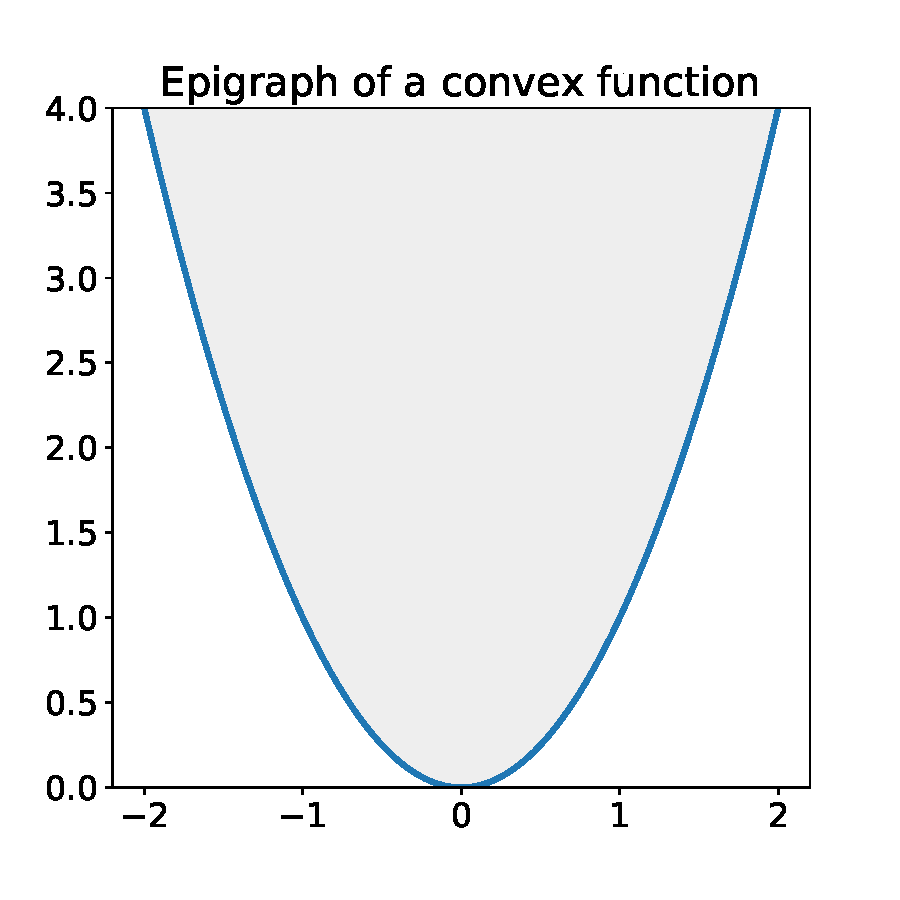
\includegraphics[width=3in]{figures/lecture1-epigraph}
\end{center}
\end{figure}
\begin{definition}

The \emph{epigraph} of a function~$f\colon \domain\to\R$ is defined as 
\[
\epi(f) = \{(x, t)\mid f(x)\le t\}\,.
\]
\end{definition}

\begin{fact}
A function is convex if and only if its epigraph is convex.
\end{fact}

Convex functions enjoy the property that local minima are also global minima. Indeed, suppose that $x\in\domain$ is a local minimum of~$f\colon\domain\to\R$ meaning that any point in a neighborhood around $x$ has larger function value. Now, for every $y\in\domain,$ we can find a small enough $\gamma$ such that
\[
f(x) \le f((1-\gamma)x+\gamma y) \le (1-\gamma)f(x)+\gamma f(y)\,.
\]
Therefore, $f(x)\le f(y)$ and so $x$ must be a global minimum.

\subsubsection{First-order characterization}

It is helpful to relate convexity to Taylor's theorem, which we recall now. We define the \emph{gradient} of a differentiable function~$f\colon\domain\to\R$ at $x\in\domain$ as the vector of partial derivatives
\[
\nabla f(x) = \left( \frac{\partial f}{\partial x_i} \right)_{i=1}^n\,.
\]
We note the following simple fact that relates linear forms of the gradient to a
one-dimensional derivative evaluated at~$0.$ It's a consequence of the multivariate chain rule.
\begin{fact}
\factlabel{1d-nd-gradient}
Assume $f\colon\domain\to\R$ is differentiable and let $x,y\in\domain.$ Then,
\[
\nabla f(x)^\trans y
= \left.\frac{\partial f(x+\gamma y)}{\partial \gamma}\right|_{\gamma=0}\,.
\]
\end{fact}
Taylor's theorem implies the following statement.
\begin{proposition}
\propositionlabel{first-order-taylor}
Assume $f\colon\domain\to\R$ is continuously differentiable along the line segment between two points $x$ and $y.$ Then,
\[
f(y) = f(x) 
+ \nabla f(x)^\trans (y-x)
+ \int_0^1 (1-\gamma)\frac{\partial^2 f(x+\gamma(y-x))}{\partial\gamma^2}\rd\gamma
\]
\end{proposition}
\begin{proof}
Apply a second order Taylor's expansion to $g(\gamma)=f(x+\gamma(y-x))$ and apply \factref{1d-nd-gradient} to the first-order term. 
\end{proof}

Among differentiable functions, convexity is equivalent to the property that the first-order Taylor approximation provides a global lower bound on the function.

\begin{figure}
\begin{center}
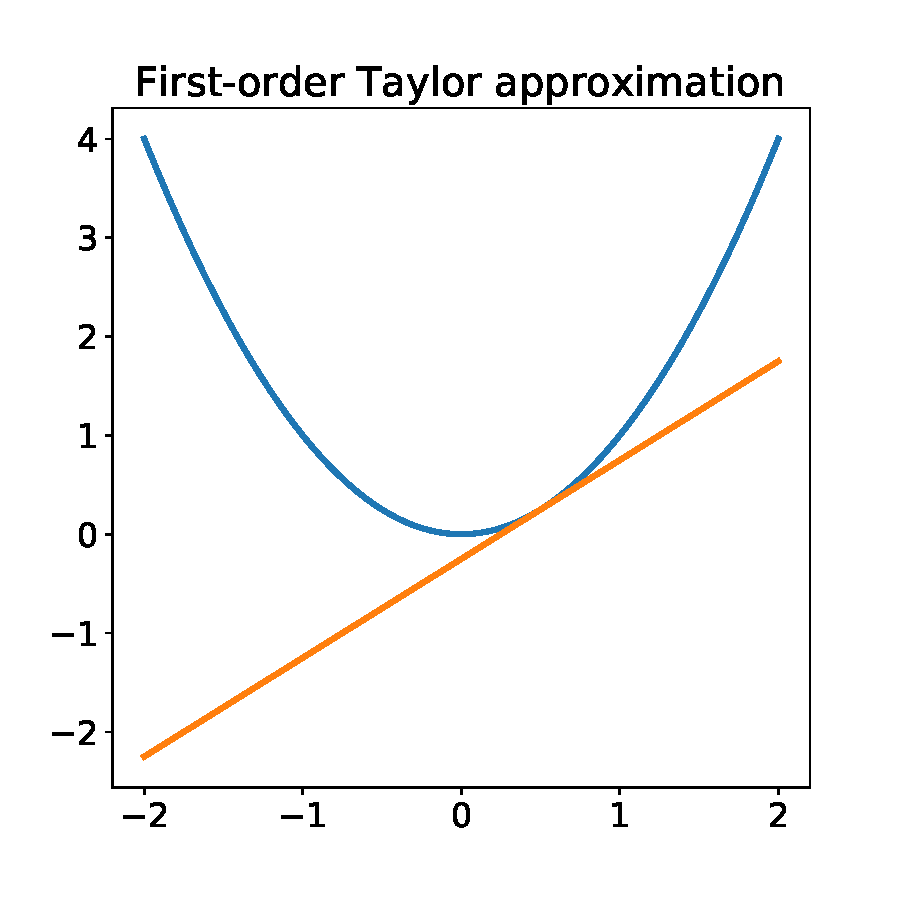
\includegraphics[width=3in]{figures/lecture1-taylor}
\end{center}
\caption{Taylor approximation of $f(x)=x^2$ at $0.5.$}
\end{figure}

\begin{proposition}
\propositionlabel{first-order-lower-bound}
Assume $f\colon\domain\to\R$ is differentiable. Then, $f$ is convex if and only if for all $x,y\in\domain$ we have
\begin{equation}\equationlabel{first-order-lower-bound}
f(y) \ge f(x) + \nabla f(x)^\trans (y-x)\,.
\end{equation}
\end{proposition}
\begin{proof}
First, suppose $f$ is convex, then by definition
\begin{align*}
f(y) &\ge \frac{f((1-\gamma)x+\gamma y)-(1-\gamma)f(x)}{\gamma}\\
&\ge f(x) +\frac{f(x+\gamma(y-x))-f(x)}\gamma\\
&\rightarrow f(x) +\nabla f(x)^\trans (y-x) \quad\text{as $\gamma\to 0$} \tag{by \factref{1d-nd-gradient}.}
\end{align*}
On the other hand, fix two points $x, y\in\domain$ and $\gamma\in[0,1]$. Putting $z=\gamma x + (1-\gamma)y$ we get from applying \equationref{first-order-lower-bound} twice,
\[
f(x) \ge f(z) + \nabla f(z)^\trans (x-z)
\quad\text{and}\quad
f(y) \ge f(z) + \nabla f(z)^\trans (y-z)
\]
Adding these inequalities scaled by $\gamma$ and $(1-\gamma)$, respectively, we get $\gamma f(x)+(1-\gamma)f(y)\ge f(z),$ which establishes convexity.
\end{proof}

A direct consequence of \propositionref{first-order-lower-bound} is that
if $\nabla f(x)=0$ vanishes at a point~$x,$ then $x$ must be a global minimizer
of~$f.$

\begin{remark}[Subgradients]
Of course, not all convex functions are differentiable. The absolute
value~$f(x)=|x|,$ for example, is convex but not differentiable at $0.$
Nonetheless, for every $x,$ we can find a vector $g$ such that
\[
f(y) \ge f(x) + g^\trans (y-x)\,.
\]
Such a vector is called a \emph{subgradient} of $f$ at $x.$ The existence of
subgradients is often sufficient for optimization.
\end{remark}

\subsubsection{Second-order characterization}

We define the \emph{Hessian} matrix of $f\colon\domain\to\R$ at a point $x\in\domain$ as the matrix of second order partial derivatives:
\[
\nabla^2 f(x) = \left( \frac{\partial^2 f}{\partial x_i\partial x_j} \right)_{i,j\in[n]}\,.
\]
Schwarz's theorem implies that the Hessian at a point $x$ is symmetric provided
that $f$ has continuous second partial derivatives in an open set around~$x.$

In analogy with \factref{1d-nd-gradient}, we can relate quadratic forms in the
Hessian matrix to one-dimensional derivatives using the chain rule.
\begin{fact}
\factlabel{1d-nd-hessian}
Assume that $f\colon\domain\to\R$ is twice differentiable along the line segment from $x$ to $y.$ Then,
\[
y^\trans \nabla^2f(x+\gamma y)y 
= \frac{\partial^2f(x+\gamma y)}{\partial\gamma^2}\,.
\]
\end{fact}

\begin{proposition}
If $f$ is twice continuously differentiable on its domain~$\domain$, then $f$ is convex if and only if $\nabla^2 f(x)\succeq 0$ for all $x\in\domain.$ 
\end{proposition}
\begin{proof}
Suppose $f$ is convex and our goal is to show that the Hessian is positive semidefinite. 
Let $y=x + \alpha u$ for some arbitrary vector~$u$ and scalar $\alpha.$
\propositionref{first-order-lower-bound} shows
\[
f(y) - f(x) -\nabla f(x)^\trans (y-x) \ge 0
\]
Hence, by \propositionref{first-order-taylor},
\begin{align*}
0&\le  \int_0^1 (1-\gamma)\frac{\partial^2 f(x+\gamma(y-x))}{\partial\gamma^2}\rd\gamma\\
&=  (1-\gamma)\frac{\partial^2 f(x+\gamma(y-x))}{\partial\gamma^2}
\quad\text{for some $\gamma\in(0,1)$} \tag{by the mean value theorem}\\
&= (1-\gamma)(y-x)^\trans \nabla^2 f(x+\gamma (y-x))(y-x) 
\tag{by \factref{1d-nd-hessian}}\,.
\end{align*}
Plugging in our choice of~$y,$ this shows $0\le u^\trans \nabla^2
f(x+\alpha\gamma u)u.$ Letting $\alpha$ tend to zero establishes that $\nabla^2
f(x)\succeq 0.$ (Note that $\gamma$ generally depends on $\alpha$ but is always
bounded by~$1.$)

Now, suppose the Hessian is positive semidefinite everywhere in $\domain$ and
our goal is to show that  the function~$f$ is convex.  Using the same derivation
as above, we can see that the second-order error term in Taylor's theorem must
be nonnegative. Hence, the first-oder approximation is
a global lower bound and so the function~$f$ is convex by
\propositionref{first-order-lower-bound}.
\end{proof}

\subsection{Convex optimization}
Much of this course will be about different ways of minimizing a convex function~$f\colon\domain\to\R$ over a convex domain~$\domain:$ 
\[
\min_{x\in \Omega} f(x)
\]
Convex optimization is not necessarily easy! 
For starters, convex sets do not necessarily enjoy compact descriptions. When solving computational problems involving convex sets, we need to worry about how to represent the convex set we're dealing with. Rather than asking for an explicit description of the set, we can instead require a computational abstraction that highlights essential operations that we can carry out. The Separation Theorem motivates an important computational abstraction called \emph{separation oracle}.

\begin{definition}
A \emph{separation oracle} for a convex set~$K$ is a device, which given any point $x\not\in K$ returns a hyperplane separating $x$ from $K.$
\end{definition}

Another computational abstraction is a \emph{first-order oracle} that given a point $x\in\domain$ returns the gradient $\nabla f(x).$ Similarly, a \emph{second-order oracle} returns $\nabla^2 f(x).$ A function value oracle or \emph{zeroth-order oracle} only returns $f(x).$
First-order methods are algorithms that make do with a first-order oracle.

\subsubsection{What is efficient?}
Classical complexity theory typically quantifies the resource consumption (primarily running time or memory) of an algorithm in terms of the bit complexity of the input. 
This approach can be cumbersome in convex optimization and most textbooks shy away from it. 
Instead, it's customary in optimization to quantify the cost of the algorithm in terms of how often it accesses one of the oracles we mentioned.

The definition of ``efficient'' is not completely cut and dry in optimization. 
Typically, our goal is to show that an algorithm finds a solution~$x$ with $f(x) = \min_{x\in\domain}f(x) + \epsilon$ for some additive error $\epsilon>0.$ 
The cost of the algorithm will depend on the target error. 
Highly practical algorithms often have a polynomial dependence on $\epsilon,$ such as $O(1/\epsilon)$ or even $O(1/\epsilon^2).$ Other algorithms achieve $O(\log(1/\epsilon))$ steps in theory, but are prohibitive in their actual computational cost. Technically, if we think of the parameter~$\epsilon$ as being part of the input, it takes only $O(\log(1/\epsilon))$ bits to describe the error parameter. Therefore, an algorithm that depends more than logarithmically on $1/\epsilon$ may not be polynomial time algorithm in its input size.

In this course, we will make an attempt to highlight both the theoretical performance and practical appeal of an algorithm. Moreover, we will discuss other performance criteria such as robustness to noise. How well an algorithm performs is rarely decided by a single criterion, and usually depends on the application at hand.

\section{Lecture 2: Gradient method}
\sectionlabel{gradient-descent}

In this lecture we encounter the fundamentally important \emph{gradient method}
and a few ways to analyze its convergence behavior.
The goal here is to solve a problem of the form
\[
\min_{x\in\domain} f(x)\,
\]
where we'll make some additional assumptions on the
function~$f\colon\domain\to\R.$ The technical exposition closely follows the
corresponding chapter in Bubeck's text~\cite{Bubeck}.

\subsection{Gradient descent}

For a differentiable function~$f,$ the basic gradient method starting from an
initial point $x_0$ is defined by the iterative description
\[
x_{t+1} = x_t - \eta \nabla_t f(x_t)\,\qquad\qquad(t\ge 0)
\]
where $\eta_t$ is the so-called \emph{step size} that may vary with~$t.$

The first assumption that leads to a convergence analysis is that the gradients
of the function aren't too big over the domain.

\begin{definition}[$L$-Lipschitz]
A differentiable function~$f$ is said to be \emph{$L$-Lipschitz} over the
domain~$\domain$ if for all~$x\in\domain,$ we have
\[
\|\nabla f(x)\| \leq L\,.
\]
\end{definition}

\begin{fact}
If a function~$f$ is $L$-Lipschitz, it implies that the difference between two points in the range is bounded,
\[
|f(x) - f(y)| \leq L \|x - y\|
\]
\end{fact}

How can we ensure that $x_{t+1}\in\domain$?  One natural approach is to
``project'' each iterate back onto the domain~$\domain.$

\begin{definition}[Projection]
The \emph{projection} of a point~$x$ onto a set $\domain$ is defined as
\[
\Pi_{\domain}(x) = \arg\min_{y\in\domain} \|x-y\|
\]
\end{definition}

\begin{example}
\examplelabel{euclidean-ball}
A projection onto the Euclidean ball $B_2$ is just normalization:
\[
\Pi_{B_2}(x) = \dfrac{x}{\|x\|}
\]
\end{example}
%
A crucial property of projections is that when $x\in\Omega,$ we have for any $y$
(possibly outside $\Omega$):
\[
\| \Pi_{\domain}(y) - x \|^2 \leq \| y - x \|^2\
\]
That is, the projection of $y$ onto a convex set containing $x$ is closer to $x$. 
%
\begin{lemma}
\lemmalabel{pythagorean}
\[
\| \Pi_{\domain}(y) - x \|^2 \leq \| y - x \|^2 - \| y - \Pi_{\domain}(y) \|^2
\]
Which follows from the Pythagorean theorem. Note that this lemma implies the above property.
\end{lemma}

\subsubsection{Modifying gradient descent with projections}

So now we can modify our original procedure to use two steps.
\[
y_{t+1} = x_t - \eta \nabla f(x_t)
\]
\[
x_{t+1} = \Pi_{\domain}(y_{t+1})
\]

And we are guaranteed that $x_{t+1}\in\domain$. Note that computing the
projection may be the hardest part of your problem, as you are computing an
$\arg\min$. However, there are convex sets for which we know explicitly how to
compute the projection (see \exampleref{euclidean-ball}).

\subsection{Convergence rate of gradient descent for Lipschitz functions}

\begin{theorem}[Projected Gradient Descent for $L$-Lipschitz Functions]
\theoremlabel{lipschitz}

Assume that function $f$ is convex, differentiable, and closed with bounded
gradients. Let $L$ be the Lipschitz constant of $f$ over the convex domain
$\Omega$. Let $R$ be the upper bound on the distance $\lVert x_1 - x^* \rVert_2$
from the initial point $x_1$ to the optimal point $x^* = \arg\min_{x \in \Omega} f(x)$.
Let $t$ be the number of iterations of project gradient descent.
If the learning rate $\eta$ is set to $\eta=\frac{R}{L\sqrt(t)}$,
then $$f\left(\frac{1}{t}\sum_{s=1}^t x_s\right) - f\left(x^*\right) \leq
\frac{RL}{\sqrt{t}}.$$
\end{theorem}

This means that the difference between the functional value of the average
point during the optimization process from the optimal value is bounded above
by a constant proportional to $\frac{1}{\sqrt{t}}$.

Before proving the theorem, recall the ``Fundamental Theorem of Optimization'',
which is that an inner product can be written as a sum of norms: $u^\trans v =
\frac{1}{2}(\lVert u \rVert^2 + \lVert v \lVert^2 - \lVert u - v \rVert^2)$.
This property can be seen from $\lVert u - v \rVert^2 = \lVert u \rVert^2 + \lVert v \lVert^2 - 2 u^\trans v$.

\begin{proof}[Proof of \theoremref{lipschitz}.]

The proof begins by first bounding the difference in function values $f(x_s) -
f(x^*)$.

\begin{align}
    f(x_s) - f(x^*) &\leq \nabla f(x_s)^\trans (x_s - x^*) \equationlabel{a} \\
    &= \frac{1}{\eta}(x_s - y_{s+1})^\trans(x_s - x^*) \equationlabel{b} \\
    &= \frac{1}{2\eta} \left(\lVert x_s - x^* \rVert^2 + \lVert x_s - y_{s+1} \rVert^2 - \lVert y_{s+1} - x^* \rVert^2 \right) \equationlabel{c} \\
    &= \frac{1}{2\eta} \left(\lVert x_s - x^* \rVert^2 - \lVert y_{s+1} - x^* \rVert^2 \right) + \frac{\eta}{2} \lVert \nabla f(x_s) \rVert^2 \equationlabel{d} \\
    &\leq \frac{1}{2\eta} \left(\lVert x_s - x^* \rVert^2 - \lVert y_{s+1} - x^* \rVert^2 \right) + \frac{\eta L^2}{2} \equationlabel{e} \\
    &\leq \frac{1}{2\eta} \left(\lVert x_s - x^* \rVert^2 - \lVert x_{s+1} - x^* \rVert^2 \right) + \frac{\eta L^2}{2} \equationlabel{f}
\end{align}

\equationref{a} comes from the definition of convexity. \equationref{b} comes
from the update rule for projected gradient descent. \equationref{c} comes from
the ``Fundamental Theorem of Optimization.'' \equationref{d} comes from the
update rule for projected gradient descent. \equationref{e} is because $f$ is
$L$-Lipschitz. \equationref{f}
comes from \lemmaref{pythagorean}.

Now, sum these differences from $s=1$ to $s=t$:

\begin{align}
   \sum_{s=1}^t f(x_s) - f(x^*) &\leq  \frac{1}{2\eta} \sum_{s=1}^t \left(\lVert x_s - x^* \rVert^2 - \lVert x_{s+1} - x^* \rVert^2 \right) + \frac{\eta L^2 t}{2} \equationlabel{g} \\
   &= \frac{1}{2\eta} \left(\lVert x_1 - x^* \rVert^2 - \lVert x_{t} - x^{*} \rVert^2 \right) + \frac{\eta L^2 t}{2} \equationlabel{h} \\
   &\leq \frac{1}{2\eta} \lVert x_1 - x^* \rVert^2 + \frac{\eta L^2 t}{2} \equationlabel{i} \\
   &\leq \frac{R^2}{2\eta} + \frac{\eta L^2 t}{2} \equationlabel{j}
\end{align}

\equationref{h} is because \equationref{g} is a telescoping sum.
\equationref{i} is because $\lVert x_{t} - x^* \rVert^2 \geq 0$.
\equationref{j} is by the assumption that $\lVert x_1 - x^* \rVert^2 \leq R^2$.

Finally,

\begin{align*}
    f\left(\frac{1}{t}\sum_{s=1}^t x_s\right) - f\left(x^*\right)
&\leq \frac{1}{t} \sum_{s=1}^t f(x_s) - f\left(x^*\right) \tag{by convexity} \\
&\leq \frac{R^2}{2\eta t} + \frac{\eta L^2}{2} \tag{by \equationref{j}}\\
&\leq \frac{RL}{\sqrt{t}} \tag{for $\eta=R/L\sqrt{t}.$}
\end{align*}

\end{proof}

\subsection{Convergence rate for smooth functions}

The next property we'll encounter is called \emph{smoothness} and it often leads
to stronger convergence guarantees.

\begin{definition}[$\beta$-smoothness]
A continuously differentiable function f is $\beta$ smooth if the gradient $\nabla f$ is $\beta$-Lipschitz, i.e
$$\|\nabla f(x) - \nabla f(y)\| \leq \beta\|x-y\|$$
\end{definition}


\begin{lemma}\label{l1}
Let $f$ be a $\beta$-smooth function on $\R^n$.  Then for any $x,y \in \R^n$, one has
$$|f(x) - f(y) - \nabla f(y)^\trans(x-y)| \leq \frac{\beta}{2}\|x-y\|^2$$
\end{lemma}

\begin{proof}
First represent $f(x) - f(y)$ as an integral, apply Cauchy-Schwarz and then $\beta$-smoothness:

\begin{align*}
|f(x) - f(y) - \nabla f(y)^\trans(x-y)|\\
&=\left|\int\limits_{0}^1 \nabla f(y + t(x-y))^\trans(x-y)dt - \nabla
f(y)^\trans(x-y)\right|\\
&\leq  \int\limits_{0}^1 \|\nabla f(y + t(x-y)) - \nabla f(y)\|\cdot \|x-y\|dt\\
&\leq \int\limits_{0}^1 \beta t\|x-y\|^2dt\\
&= \frac{\beta}{2}\|x-y\|^2\\
\end{align*}
\end{proof}

We also need the following lemma.

\begin{lemma} \label{lm2}
Let $f$ be a $\beta$-smooth function, then for any $x,y \in \R^n$, one has
$$f(x) - f(y)\leq \nabla f(x)^\trans(x-y) - \frac{1}{2\beta}\|\nabla f(x) - \nabla f(y)\|$$
\end{lemma}

\begin{proof}
Let $z = y - \frac{1}{\beta}(\nabla f(y) - \nabla f(x))$.  Then one has

$$f(x) - f(y)$$
\begin{align}
    &= f(x) - f(z) + f(z) - f(y) \\
    &\leq \nabla f(x)^\trans(x-z) + \nabla f(y)^\trans(z-y) + \frac{\beta}{2}\|z-y\|^2 \\
    &= \nabla f(x)^\trans(x-y) + (\nabla f(x) - \nabla f(y))^\trans(y-z) + \frac{1}{2\beta}\|\nabla f(x) - \nabla f(y)\|^2 \\
    &= \nabla f(x)^\trans(x-y) - \frac{1}{2\beta} \|\nabla f(x) - \nabla f(y)\|^2
\end{align}

\end{proof}


We will show that gradient descent with the update rule
$$x_{t+1} = x_t - \eta \nabla f(x_t)$$
attains a faster rate of convergence under the smoothness condition.

\begin{theorem}
Let $f$ be convex and $\beta$-smooth on $\R^n$ then gradient descent with $\eta = \frac{1}{\beta}$ satisfies
$$f(x_t) - f(x^*) \leq \frac{2\beta\|x_1 - x^*\|^2}{t-1}$$
\end{theorem}
To prove this we will need the following two lemmas.

\begin{proof}
By the update rule and lemma \ref{l1} we have
$$f(x_{s+1}) - f(x_s) \leq -\frac{1}{2\beta}\|\nabla f(x_s)\|^2 $$
In particular, denoting $\delta_s = f(x_s) - f(x^*)$ this shows
$$\delta_{s+1} \leq \delta_s - \frac{1}{2\beta}\|\nabla f(x_s)\|^2 $$
One also has by convexity
$$\delta_s \leq \nabla f(x)s)^\trans(x_s - x^*) \leq \|x_s - x^*\| \cdot \|\nabla f(x_s)\|$$
We will prove that $\|x_s - x^*\|$ is decreasing with $s$, which with the two above displays will imply
$$\delta_{s+1}\leq \delta_s - \frac{1}{2\beta\|x_1 - x^*\|^2}\delta_s^2$$
We solve the recurrence as follows.  Let $w = \frac{1}{2\beta\|x_1 - x^*\|^2}$, then
$$w\delta_s^2 + \delta_{s+1} \leq \delta_s \iff w\frac{\delta_s}{\delta_{s+1}} + \frac
{1}{\delta_s} \leq \frac{1}{\delta_{s+1}} \implies \frac{1}{\delta_{s+1}} - \frac{1}{\delta_s} \geq w \implies \frac{1}{\delta_t} \geq w(t-1)$$
To finish the proof it remains to show that $\|x_s - x^*\|$ is decreasing with $s$.  Using lemma \ref{lm2} one immediately gets
$$ (\nabla f(x) - \nabla f(y))^\trans(x - y) \geq \frac{1}{\beta} \|\nabla f(x) - \nabla f(y)\|^2$$
We use this and the fact that $\nabla f(x^*) = 0$
\begin{align}
    \|x_{s+1} - x^*\|^2 &= \|x_s - \frac{1}{\beta}\nabla f(x_s) - x^*\|^2 \\
    &= \|x_s - x^*\|^2 - \frac{2}{\beta}\nabla f(x_s)^\trans(x_s - x^*) + \frac{1}{\beta^2}\|\nabla f(x_s)\|^2 \\
    &\leq \|x_s - x^*\|^2 - \frac{1}{\beta^2} \|\nabla f(x_s)\|^2 \\
    &\leq \|x_s - x^*\|^2
\end{align}
which concludes the proof.
\end{proof}


\section{Lecture 3: Strong convexity}
\sectionlabel{strongconvexity}

This lecture introduces the notion of $\alpha$-strong convexity and combines it
with $\beta$-smoothness to develop the concept of condition number.  Adding an
assumption of, respectively, strong convexity or conditioning improves the rates
of error decay for gradient descent proved in the previous lecture from
$O(1/\sqrt{t})$ to $O(1/t)$ and $O(1/t)$ to $O(\mathrm{e}^{-t})$.

The technical part follows the corresponding chapter in Bubeck's
text~\cite{Bubeck}.

\subsection{Reminders}

Recall that we had (at least) two definitions apiece for convexity and
smoothness: a general definition for all functions and a more compact definition
for (twice-)differentiable functions.

A function $f$ is convex if, for each input, there exists a globally valid
\emph{linear} lower bound on the function: $f(y) \geq f(x) + g^\trans(x)(y-x)$.
For differentiable functions, the role of $g$ is played by the gradient.

A function $f$ is $\beta$-smooth if, for each input, there exists a globally
valid \emph{quadratic} upper bound on the function, with (finite) quadratic
parameter $\beta$: $f(y) \leq f(x) + g^\trans(x)(y-x) +
\frac{\beta}{2}\Norm{x-y}^2$.  More poetically, a smooth, convex function is
``trapped between a parabola and a line''.  Since $\beta$ is covariant with
affine transformations, e.g. changes of units of measurement, we will frequently
refer to a $\beta$-smooth function as simply smooth.

For twice-differentiable functions, these properties admit simple conditions for
smoothness in terms of the Hessian, or matrix of second partial derivatives.  A
$\mathcal{D}^2$ function $f$ is convex if $\nabla^2f(x) \succeq 0$ and it is
$\beta$-smooth if $\nabla^2f(x) \preceq \beta I$.

We furthermore defined the notion of $L$-Lipschitzness.  A function $f$ is
$L$-Lipschitz if the amount that it ``stretches'' its inputs is bounded by $L$:
$\Abs{f(x)-f(y)} \leq L\Norm{x-y}$.  Note that for differentiable functions,
$\beta$-smoothness is equivalent to $\beta$-Lipschitzness of the gradient.

\subsection{Strong convexity}

With these three concepts, we were able to prove two error decay rates for
gradient descent (and its projective, stochastic, and subgradient flavors).
However, these rates were substantially slower than what's observed in certain
settings in practice.

Noting the asymmetry between our linear lower bound (from convexity) and our
quadratic upper bound (from smoothness) we introduce a new, more restricted
function class by upgrading our lower bound to second order.

\begin{definition}[$\alpha$-Strong Convexity]
A function $f\colon\domain\to\R$
is \emph{$\alpha$-strongly convex}
if, for all $x,y\in\domain$,
the following inequality holds
for some $\alpha>0$:
\[
f(y) \geq f(x) + g(x)^\trans(y-x) + \frac{\alpha}{2}\Norm{x-y}^2
\]
\end{definition}

As with smoothness, we will often shorten ``$\alpha$-strongly convex'' to
``strongly convex''.  A strongly convex, smooth function is one that can be
``squeezed between two parabolas''.  If $\beta$-smoothness is a good thing, then
$\alpha$-convexity guarantees we don't have too much of a good thing.

Once again, twice-differentiable functions afford a quick condition: a $D^2$
function is $alpha$-strongly convex if $\nabla^2f(x) \succeq \alpha I$.

Once again, note that $\alpha$ changes under affine transformations.
Conveniently enough, for $\alpha$-strongly convex, $\beta$-smooth functions, we
can define a basis-independent quantity that combines these properties:

\begin{definition}[Condition Number]
An $\alpha$-strongly convex, $\beta$-smooth function $f$
has \emph{condition number} $\frac{\beta}{\alpha}$.
\end{definition}

For a positive-definite quadratic function $f$, this definition of the condition
number corresponds with the perhaps more familiar definition of the condition
number of a matrix.

\subsection{A look back and ahead}

The following table summarizes the results from the previous lecture and the
results to be obtained in this lecture.  In both, the value~$\epsilon$ is the
difference between $f$ at some value $x'$ computed from the outputs of gradient
descent and $f$ calculated at an optimizer $x^*$.

\begin{table}[h]
    \centering
    \begin{tabular}{|r|c|c|}
        \hline
         & Convex & Strongly Convex\\
        \hline
         Lipschitz & $\epsilon \leq O(1/\sqrt{t})$
         & $\epsilon \leq O(1/t)$ \\
         \hline
         Smooth & $\epsilon \leq O(1/t)$
         & $\epsilon \leq O(\mathrm{e}^{-t})$ \\
         \hline
    \end{tabular}
    \caption{Bounds on error $\epsilon$
    as a function of number of steps taken $t$
    for gradient descent applied to various classes of functions.}
    \label{tab:proofs}
\end{table}

Since a rate that is exponential in terms of the magnitude of the error is
linear in terms of the bit precision, this rate of convergence is termed
\emph{linear}.  We now move to prove these rates.

\subsection{Convergence rate strongly convex functions}

\begin{theorem}\theoremlabel{convergence_strongconvexity} 
Assume $f\colon\domain\to\R$ is \emph{$\alpha$-strongly convex} and
\emph{$L$-Lipschitz}. Let $x^{*}$ be an optimizer of $f$, and let $x_{s}$ be the
updated point at step $s$ using projected gradient descent. Let the max number
of iterations be $t$ with an adaptive step size $\eta_{s} =
\frac{2}{\alpha(s+1)}$, then 
\[
f\left(\sum_{s=1}^{t}\frac{2s}{t(t+1)}x_{s}\right) - f(x^{*})\leq\frac{2 L^{2}}{\alpha(t+1)}
\]
\end{theorem}

The theorem implies the convergence rate of projected gradient descent for
$\alpha$-strongly convex functions is similar to that of $\beta$-smooth
functions with a bound on error $\epsilon \leq O(1/t)$.  In order to prove
\theoremref{convergence_strongconvexity}, we need the following proposition.

\begin{proposition}[Jensen's inequality]\propositionlabel{jensen_inequality}
Assume $f\colon\domain\to\R$ is a convex function and $x_{1}, x_{2}, ...,$\\
$,x_{n},\sum_{i=1}^{n}\gamma_{i}x_{i}/\sum_{i=1}^{n}\gamma_{i}\in\domain$ with weights $\gamma_{i} > 0$, then
\[
f\left(\frac{\sum_{i=1}^{n}\gamma_{i}x_{i}}{\sum_{i=1}^{n}\gamma_{i}}\right) \leq \frac{\sum_{i=1}^{n}\gamma_{i}f(x_{i})}{\sum_{i=1}^{n}\gamma_{i}}
\]
\end{proposition}

For a graphical  ``proof'' follow
\href{http://mark.reid.name/blog/behold-jensens-inequality.html}{this link}.

\begin{proof}[Proof of \theoremref{convergence_strongconvexity}.] 
Recall the two steps update rule of projected gradient descent
\begin{align*}
y_{s+1} &= x_{s} - \eta_{s}\nabla f(x_{s})\\
x_{s+1} &= \Pi_{\domain}(y_{s+1})
\end{align*}

First, the proof begins by exploring an upper bound of difference between function values $f(x_{s})$ and $f(x^{*})$.
\begin{align*}
f(x_{s}) - f(x^{*}) &\leq \nabla f(x_{s})^{\trans}(x_{s}-x^{*}) - \frac{\alpha}{2}\|x_{s}-x^{*}\|^{2}\\
			 &=\frac{1}{\eta_{s}} (x_{s} - y_{s+1})^{\trans}(x_{s}-x^{*}) - \frac{\alpha}{2}\|x_{s}-x^{*}\|^{2} \tag{by update rule}\\ 
			 &=\frac{1}{2\eta_{s}} (\|x_{s} - x^{*}\|^{2} + \|x_{s} - y_{s+1}\|^{2} - \|y_{s+1}-x^{*}\|^{2}) - \frac{\alpha}{2}\|x_{s}-x^{*}\|^{2} \tag{by "Fundamental Theorem of Optimization"}\\
			 &=\frac{1}{2\eta_{s}} (\|x_{s} - x^{*}\|^{2} - \|y_{s+1}-x^{*}\|^{2}) +\frac{\eta_{s}}{2}\|\nabla f(x_{s})\|^{2} - \frac{\alpha}{2}\|x_{s}-x^{*}\|^{2} \tag{by update rule}\\
			 &\leq \frac{1}{2\eta_{s}} (\|x_{s} - x^{*}\|^{2} - \|x_{s+1}-x^{*}\|^{2}) +\frac{\eta_{s}}{2}\|\nabla f(x_{s})\|^{2} - \frac{\alpha}{2}\|x_{s}-x^{*}\|^{2} \tag{by \lemmaref{pythagorean}}\\
			 &\leq (\frac{1}{2\eta_{s}} - \frac{\alpha}{2})\|x_{s}-x^{*}\|^{2} -\frac{1}{2\eta_{s}}\|x_{s+1}-x^{*}\|^{2} + \frac{\eta_{s}L^{2}}{2} \tag{by Lipschitzness}
\end{align*}
By multiplying $s$ on both sides and substituting the step size $\eta_{s}$ by $\frac{2}{\alpha(s+1)}$, we get
\[
s(f(x_{s}) - f(x^{*})) \leq \frac{L^{2}}{\alpha} + \frac{\alpha}{4}(s(s-1)\|x_{s}-x^{*}\|^{2} - s(s+1)\|x_{s+1} - x^{*}\|^{2})
\]
Finally, we can find the upper bound of the function value shown in \theoremref{convergence_strongconvexity} obtained using $t$ steps projected gradient descent
\begin{align*}
f\left(\sum_{s=1}^{t}\frac{2s}{t(t+1)}x_{s}\right)
&\leq \sum_{s=1}^{t}\frac{2s}{t(t+1)}f(x_{s}) 
\tag{by \propositionref{jensen_inequality}}\\
&\leq \frac{2}{t(t+1)}\sum_{s=1}^{t}\left(sf(x^{*}) + \frac{L^{2}}{\alpha} 
+  \frac{\alpha}{4}(s(s-1)\|x_{s}-x^{*}\|^{2} - s(s+1)\|x_{s+1} - x^{*}\|^{2}) \right)\\
&= \frac{2}{t(t+1)}\sum_{s=1}^{t}sf(x^{*}) + \frac{2L^{2}}{\alpha(t+1)} - \frac{\alpha}{2}\|x_{t+1} - x^{*}\|^{2} \tag{by telescoping sum}\\
&\leq f(x^{*}) + \frac{2L^{2}}{\alpha(t+1)}
\end{align*}

This concludes that solving an optimization problem with a strongly convex
objective function with projected gradient descent has a convergence rate is of
the order $\frac{1}{t+1}$, which is faster compared to the case purely with
Lipschitzness.
\end{proof}


\subsection{Convergence rate for smooth and strongly convex functions}

\begin{theorem}\theoremlabel{convergence_smooth_and_strongconvexity} 
Assume $f\colon\R^n\to\R$ is \emph{$\alpha$-strongly convex} and
\emph{$\beta$-smooth}. Let $x^{*}$ be an optimizer of $f$, and let $x_{t}$ be
the updated point at step $t$ using gradient descent with a constant step size
$\frac{1}{\beta}$, i.e. using the update rule $x_{t+1} = x_t -
\frac{1}{\beta}\nabla f(x_t)$. Then,
\[
\|x_{t+1} - x^*\|^2 \leq \exp{(-t \frac{\alpha}{\beta})}\|x_1 - x^*\|^2
\]
\end{theorem}

In order to prove \theoremref{convergence_smooth_and_strongconvexity}, we
require use of the following lemma. 
%
\begin{lemma}\lemmalabel{smooth_strong_convex_f_diff}
Assume $f$ as in \theoremref{convergence_smooth_and_strongconvexity}. Then
$\forall x,y \in \R^n$ and an update of the form $x^+ = x -
\frac{1}{\beta}\nabla f(x)$, 
\[ 
f(x^+) - f(y) \leq \nabla f(x)^\trans (x-y) -
\frac{1}{2\beta}\|\nabla f(x)\|^2 - \frac{\alpha}{2}\|x-y\|^2
\]
\end{lemma}
\begin{proof}[Proof of \lemmaref{smooth_strong_convex_f_diff}.]
    \begin{align*}
        f(x^+) - f(x) + f(x) - f(y) &\leq \nabla f(x)^\trans (x^+ - x) + \frac{\beta}{2}\|x^+ - x\|^2 \tag{Smoothness} \\
        & \quad \ + \nabla f(x)^\trans (x-y) - \frac{\alpha}{2}\|x-y\|^2 \tag{Strong convexity} \\
        &= \nabla f(x)^\trans(x^+ - y) + \frac{1}{2\beta}\|\nabla f(x)\|^2 - \frac{\alpha}{2}\|x-y\|^2 \tag{Definition of $x^+$} \\
        &= \nabla f(x)^\trans (x - y) - \frac{1}{2\beta}\|\nabla f(x)\|^2 - \frac{\alpha}{2}\|x-y\|^2 \tag{Definition of $x^+$}
    \end{align*}
\end{proof}
Now with \lemmaref{smooth_strong_convex_f_diff} we are able to prove  \theoremref{convergence_smooth_and_strongconvexity}.
\begin{proof}[Proof of \theoremref{convergence_smooth_and_strongconvexity}.]
\begin{align*}
    \|x_{t+1} -x^*\|^2 &= \|x_t - \frac{1}{\beta}\nabla f(x_t) - x^*\|^2 \\
    &= \|x_t-x^*\|^2 - \frac{2}{\beta} \nabla f(x_t)^\trans(x_t - x^*) + \frac{1}{\beta^2}\|\nabla f(x_t)\|^2 \\
    &\leq (1-\frac{\alpha}{\beta})\|x_t-x^*\|^2 \tag{Use of \lemmaref{smooth_strong_convex_f_diff} with $y=x^*$, $x=x_t$}\\
    &\leq (1-\frac{\alpha}{\beta})^t \|x_1-x^*\|^2 \\ 
    &\leq \exp{(-t \frac{\alpha}{\beta})} \|x_1-x^*\|^2
\end{align*}
\end{proof}

We can also prove the same result for the constrained case using projected
gradient descent.

\begin{theorem}\theoremlabel{constrained_convergence_smooth_and_strongconvexity} 
Assume $f\colon\domain\to\R$ is \emph{$\alpha$-strongly convex} and
\emph{$\beta$-smooth}. Let $x^{*}$ be an optimizer of $f$, and let $x_{t}$ be
the updated point at step $t$ using projected gradient descent with a constant
step size $\frac{1}{\beta}$, i.e. using the update rule $x_{t+1} =
\Pi_{\domain}(x_{t} - \frac{1}{\beta}\nabla f(x_{t}))$ where $\Pi_{\domain}$ is
the projection operator. Then, 
\[
\|x_{t+1} - x^*\|^2 \leq \exp{(-t \frac{\alpha}{\beta})}\|x_1 - x^*\|^2
\]
\end{theorem}
As in \theoremref{convergence_smooth_and_strongconvexity}, we will require the
use of the following Lemma in order to prove
\theoremref{constrained_convergence_smooth_and_strongconvexity}. 

\begin{lemma}\lemmalabel{constrained_smooth_strong_convex_f_diff}
    Assume $f$ as in \theoremref{convergence_smooth_and_strongconvexity}. Then $\forall x,y \in \domain$, define $x^+\in\domain$ as $x^+ = \Pi_{\domain}(x - \frac{1}{\beta}\nabla f(x))$ and the function $g\colon\domain\to\R$ as $g(x) = \beta(x-x^+)$. Then
    \[
        f(x^+) - f(y) \leq g(x)^\trans (x-y) - \frac{1}{2\beta}\|g(x)\|^2 - \frac{\alpha}{2}\|x-y\|^2
    \]
\end{lemma}

\begin{proof}[Proof of \lemmaref{constrained_smooth_strong_convex_f_diff}.]
    The following is given by the Projection Lemma, for all $x,x^+,y$ defined as in \theoremref{constrained_convergence_smooth_and_strongconvexity}.
    \begin{align*}
        \nabla f(x)^\trans (x^+ - y) &\leq g(x)^\trans(x^+ - y)
    \end{align*}
    Therefore, following the form of the proof of \lemmaref{smooth_strong_convex_f_diff},
    \begin{align*}
        f(x^+) - f(x) + f(x) - f(y) &\leq \nabla f(x)^\trans(x^+-y) + \frac{1}{2\beta}\|\nabla g(x)\|^2 - \frac{\alpha}{2}\|x-y\|^2\\
        &\leq \nabla g(x)^\trans(x^+-y) + \frac{1}{2\beta}\|\nabla g(x)\|^2 - \frac{\alpha}{2}\|x-y\|^2\\
        &= \nabla g(x)^\trans(x-y) - \frac{1}{2\beta}\|\nabla g(x)\|^2 -
\frac{\alpha}{2}\|x-y\|^2\qedhere
    \end{align*}
\end{proof}

The proof of \theoremref{constrained_convergence_smooth_and_strongconvexity} is
exactly as in \theoremref{convergence_smooth_and_strongconvexity} after
substituting the appropriate projected gradient descent update in place of the
standard gradient descent update, with
\lemmaref{constrained_smooth_strong_convex_f_diff} used in place of
\lemmaref{smooth_strong_convex_f_diff}. 

\section{Lecture 4: Some applications of gradient methods}
\sectionlabel{applications}

This lecture was a sequence of code examples that you can find here:

\begin{center}
{\Large
\href{https://ee227c.github.io/code/lecture4.html}{Lecture 4}
}

(opens in your browser)
\end{center}



\section{Lecture 5: Conditional gradient method (Frank-Wolfe)}
\sectionlabel{frankwolfe}

In this lecture we discuss the conditional gradient method, also known as the
Frank-Wolfe (FW) algorithm~\cite{Frank1956}. The motivation for this approach is
that the projection step in projected gradient descent can be computationally
inefficient in certain scenarios. The conditional gradient method provides an
appealing alternative.

\subsection{The algorithm}
Conditional gradient side steps the projection step using a clever idea.

We start from some point~$x_0\in\domain$. Then, for time steps $t = 1$ to $T$, 
where $T$ is our final time step, we set
\[
x_{t+1} = x_t + \eta_t(\bar{x_t}-x_t)
\]
where
$$ \bar{x_t} = \arg\min_{x\in \domain} f(x_t) + \nabla f(x_t) ^\trans (x-x_t).$$
This expression simplifies to:
$$ \bar{x_t} = \arg\min_{x\in \domain} \nabla f(x_t) ^\trans x $$
Note that we need step size $\eta_t \in [0,1]$ to guarantee $x_{t+1} \in \domain$.

So, rather than taking a gradient step and projecting onto the constraint set.
We optimize a liner function (defined by the gradient) inside the constraint
set.

\subsection{Conditional gradient convergence analysis}

As it turns out, conditional gradient enjoys a convergence guarantee similar to
the one we saw for projected gradient descent.

\begin{theorem}[Convergence Analysis]
\theoremlabel{convergence}
Assume we have a function $f\colon\domain\to\R$ that is convex, $\beta$-smooth
and attains its global minimum at a point~$x^*\in\domain.$ Then, Frank-Wolfe achieves
$$ f(x_t) - f(x^*) \leq \frac{2\beta D^2}{t+2}$$
with step size $$\eta_t = \frac{2}{t+2}.$$
Here, $D$ is the diameter of $\domain$, defined as
$ D = \max_{x-y \in \domain} \| x-y \|.$ 
\end{theorem}
Note that we can trade our assumption of the existence of $x^*$ for a dependence on $L$, the Lipschitz constant, in our bound.

\begin{proof}[Proof of \theoremref{convergence}.]
By smoothness and convexity, we have
$$ f(y) \leq f(x) +\nabla f(x) ^\trans (x-x_t) + \frac{\beta}{2} \| x-y \| ^2 $$
Letting $ y = x_{t+1} $ and $x= x_t$, combined with the progress rule of conditional gradient descent, the above equation yields:
$$ f(x_{t+1}) \leq f(x_t) + \eta_t \nabla f(x_t) ^\trans (\bar{x_t} - x_t) + \frac{\eta_t^2\beta}{2} \| \bar{x_t} - x_t \| ^2 $$
We now recall the definition of $D$ from \theoremref{convergence} and observe that $\| \bar{x_t} - x_t \| ^2 \leq D^2$. Thus, we rewrite the inequality:
$$ f(x_{t+1}) \leq f(x_t) + \eta_t \nabla f(x_t) ^\trans (x_t^* - x_t) + \frac{\eta_t^2\beta D ^2}{2} $$
Because of convexity, we also have that
$$ \nabla f(x_t) ^\trans (x^*-x_t) \leq f(x^*) - f(x_t) $$
Thus,
\begin{equation}\equationlabel{convergenceInequal}
f(x_{t+1})-f(x^*) \leq (1-\eta_t)(f(x_t)-f(x^*)) + \frac{\eta_t^2\beta D ^2}{2}
\end{equation}
We use induction in order to prove $f(x_t)-f(x^*) \leq \frac{2\beta D^2}{t+2}$  based on \equationref{convergenceInequal} above.\\
First step: Base Case $t=0$ \\
Since $ f(x_{t+1})-f(x^*) \leq (1-\eta_t)(f(x_t)-f(x^*)) + \frac{\eta_t^2\beta D ^2}{2}$, when t=0, $\eta_t =\frac{2}{0+2}=1, then $
\begin{align*} f(x_1)-f(x^*) &\leq (1-\eta_t)(f(x_t)-f(x^*)) + \frac{\beta}{2}\| x_1-x^* \|^2 \\
&= (1-1)(f(x_t)-f(x^*)) + \frac{\beta}{2}\| x_1-x^* \|^2 \\
&\leq \frac{\beta D^2}{2}\\
&\leq \frac{2\beta D^2}{3}
\end{align*}
Thus, the induction hypothesis holds for our base case.

Proceeding by induction,
we assume that $f(x_t)-f(x^*) \leq \frac{2\beta D^2}{t+2}$ holds for all
integers up to $t$ and we show the claim for $t+1.$

By \equationref{convergenceInequal},
\begin{align*} f(x_{t+1})-f(x^*) &\leq \left(1- \frac{2}{t+2}\right) (f(x_t)-f(x^*))+ \frac{4}{2(t+2)} \beta D^2 \\
& \leq \left(1- \frac{2}{t+2}\right)\frac{2\beta D^2}{t+2}
+ \frac{4}{2(t+2)} \beta D^2 \\
& = \beta D^2 \left(\frac{2t}{(t+2)^2}+\frac{2}{(t+2)^2}\right) \\
& = 2\beta D^2 \cdot\frac{t+1}{(t+2)^2} \\
& = 2\beta D^2 \cdot\frac{t+1}{t+2}\cdot\frac{1}{t+2} \\
& \leq 2\beta D^2 \cdot\frac{t+2}{t+3}\cdot\frac{1}{t+2} \\
& = 2\beta D^2 \frac{1}{t+3}
\end{align*}
Thus, the inequality also holds for the $t+1$ case.

\end{proof}

\subsection{Application to nuclear norm optimization problems}

The code for the following examples can be found \href{https://ee227c.github.io/code/lecture5.html}{here}.

\subsubsection{Nuclear norm projection}
The \textit{nuclear norm} (sometimes called \textit{Schatten $1$-norm} or \textit{trace norm}) of a matrix $A$, denoted $\|A\|_*$, is defined as the sum of its singular values
\[
\|A\|_* = \sum_i \sigma_i(A)\,.
\]
The norm can be computed from the singular value decomposition of $A$.
We denote the unit ball of the nuclear norm by 
\[
B_*^{m\times n}=\{A\in\mathbb{R}^{m\times n} \mid \|A\|_*\le 1\}.
\]
How can we project a matrix $A$ onto $B_*$? Formally, we want to solve
\[
\min_{X\in B_*}\|A-X\|_F^2
\]
Due to the rotational invariance of the Frobenius norm, the solution is obtained by projecting the singular values onto the unit simplex. This operation corresponds to shifting all singular values by the same parameter $\theta$ and clipping values at $0$ so that the sum of the shifted and clipped values is equal to $1$. This algorithm can be found in \cite{Duchi2008}.

\subsubsection{Low-rank matrix completion}

Suppose we have a partially observable matrix $Y$, of which the missing entries are filled with 0 and we would like to find its completion form projected on a nuclear norm ball. Formally we have the objective function
\[
\min_{X\in B_*}\frac{1}{2}\|Y-P_O(X)|_F^2
\]
where $P_O$ is a linear projection onto a subset of coordinates of $X$ specified by $O$. In this example $P_O(X)$ will generate a matrix with corresponding observable entries as in $Y$ while other entries being 0. We can have $P_O(X) = X \odot O$ where $O$ is a matrix with binary entries.
Calculate the gradient of this function we will have
\[
\nabla f(X) = Y-X \odot O
\]
We can use projected gradient descent to solve this problem but it is more efficient to use Frank-Wolfe algorithm. We need to solve the linear optimization oracle
\[
\bar{X}_t\in \argmin_{X\in{B_*}}\nabla f(X_t)^\trans X
\]

To simplify this problem, we need a simple fact that follows from the singular
value decomposition.
%
\begin{fact}
\factlabel{fact}
The unit ball of the nuclear norm is the convex hull of rank-$1$ matrices
\[
\mathrm{conv}\{uv^\trans|\|u\|=\|v\|=1, u\in\R^m, v\in\R^n\}
=\{X\in\R^{m\times n}\mid \|X\|_*=1\}\,.
\]
\end{fact}

From this fact it follows that the minimum of $\nabla f(X_t)^\top X$ is attained
at a rank-$1$ matrix $uv^\top$ for unit vectors $u$ and $v$. 
Equivalently, we can maximize $-\nabla f(X_t)^\top uv^\top$ 
over all unit vectors~$u$ and~$v.$ Put
$Z = -\nabla f(X_T)$ and note that
\[
Z^\top uv^\top = \tr(Z^\top uv^\top) = \tr(u^\top Z v) = u^\top Z v\,.
\]

Another way to see this is to note that 
the dual norm of a nuclear norm is operator norm,
\[
\|Z\| = \max_{\|X\|_*\leq 1}\langle Z, X\rangle\,.
\]

Either way, we see that to run Frank-Wolfe over the nuclear norm ball we only
need a way to compute the top left and singular vectors of a matrix. One way of
doing this is using the classical power method:

\begin{itemize}
\item Pick a random unit vector $x_1$ and let $y_1 = A^\trans x/\|A^\trans x\|.$
\item From $k=1$ to $k=T-1:$
\begin{itemize}
\item Put $x_{k+1}=\frac{Ay_k}{\|Ay_k\|}$
\item Put $y_{k+1}=\frac{A^\trans x_{k+1}}{\|A^\trans x_{k+1}\|}$
\end{itemize}
\item Return $x_T$ and $y_T$ 
as approximate top left and right singular vectors.
\end{itemize}

\part{Krylov methods}
\section{Lecture 6: Discovering acceleration}

In this lecture, we seek to find methods that converge faster than those
discussed in previous lectures. To derive this accelerated method, we start by
considering the special case of optimizing quadratic functions. Our exposition
loosely follows Chapter~$17$ in Lax's excellent text~\cite{lax}.

\subsection{Quadratics}

\begin{definition}[Quadratic function] A quadratic function $f\colon\R^n \to \R$ takes the form: 
\begin{equation*}
f(x) = \frac{1}{2}x^T A x - b^T x + c,
\end{equation*}
where $A \in S^n$, $b \in \R^n$ and $c \in \R$.
\end{definition}

%\begin{remark}
Note that substituting $n=1$ into the above definition recovers the familiar univariate quadratic function $f(x) = ax^2 + bx + c$ where $a, b, c \in \R$, as expected. There is one subtlety in this definition: we restrict $A$ to be symmetric. In fact, we could allow $A \in \R^{n \times n}$ and this would define the same class of functions, since for any $A \in \R^{n \times n}$ there is a symmetric matrix $\tilde{A} = \frac{1}{2}\left(A + A^T\right)$ for which:
\begin{equation*}
x^TAx = x^T \tilde{A} x\ \forall x \in \R^n.
\end{equation*}
Restricting $A \in S^n$ ensures each quadratic function has a \textit{unique} representation.

The gradient and Hessian of a general quadratic function take the form:
\begin{align*}
\nabla f(x) &= Ax - b \\
\nabla^2 f(x) &= A.
\end{align*}
Note provided $A$ is non-singular, the quadratic has a unique critical point at:
\begin{equation*}
x^* = A^{-1}b.
\end{equation*}
When $A \succ 0$, the quadratic is \textit{strictly convex} and this point is the unique global minima.

\subsection{Gradient descent on a quadratic}
In this section we will consider a quadratic $f(x)$ where $A$ is positive definite, and in particular that:
\begin{equation*}
\alpha I \preceq A \preceq \beta I,
\end{equation*}
for some $0 < \alpha < \beta$. This implies that $f$ is $\alpha$-strongly convex and $\beta$-smooth. 

From \theoremref{constrained_convergence_smooth_and_strongconvexity} we know that under these conditions, gradient descent with the appropriate step size converges linearly at the rate $\exp\left(-t \frac{\alpha}{\beta}\right)$. Clearly the size of $\frac{\alpha}{\beta}$ can dramatically affect the convergence guarantee. In fact, in the case of a quadratic, this is related to the \textit{condition number} of the matrix $A$.

\begin{definition}[Condition number]
Let $A$ be a real matrix. Its \textit{condition number} (with respect to the Euclidean norm) is:
\begin{equation*}
\kappa(A) = \frac{\sigma_{\max}(A)}{\sigma_{\min}(A)},
\end{equation*}
the ratio of its largest and smallest eigenvalues.
\end{definition}

So in particular, we have that $\kappa(A) \leq \frac{\beta}{\alpha}$; henceforth, we will assume that $\alpha, \beta$ correspond to the minimal and maximal eigenvalues of $A$ so that $\kappa(A) = \frac{\beta}{\alpha}$. It follows that gradient descent with a constant step size $\frac{1}{\beta}$ converges at:
\begin{equation*}
\left||x_{t+1} - x^*\right\|^2 \leq \exp{\left(-t \frac{1}{\kappa}\right)}\|x_1 - x^*\|^2.
\end{equation*}
In many cases, $f$ is ill-conditioned and $\kappa$ can easily take values in the hundreds or thousands. In this case, case convergence could be very slow: note that at $t > \kappa$, the error may have been reduced by only a factor of $3\times$. Can we do better than this?

In the case of a quadratic, we can of course use the analytic solution $x^* = A^{-1}b$. However, it will prove instructive to consider applying gradient descent to quadratic functions, and derive the convergence bound that we previously proved for any strongly convex smooth functions. This exercise will show us where we are losing performance, and suggest a method that can attain better guarantees.

\subsubsection{Convergence analysis}

\begin{theorem}
Assume $f\colon\R^n\to\R$ is a quadratic where the quadratic coefficient matrix has a condition number $\kappa$. Let $x^{*}$ be an optimizer of $f$, and let $x_{t}$ be the updated point at step $t$ using gradient descent with a constant step size $\frac{1}{\beta}$, i.e. using the update rule $x_{t+1} = x_t - \frac{1}{\beta}\nabla f(x_t)$. Then:
\begin{equation*}
\|x_{t+1} - x^*\|^2 \leq \exp\left(-t \frac{1}{\kappa}\right)\|x_1 - x^*\|^2.
\end{equation*}
\end{theorem}
\begin{proof}
Write:
\[
f(x) = \frac{1}{2}x^T A x - b^T x + c,
\]
where $A \in S^n$, $b \in \R^n$ and $c \in \R$. A gradient descent update with step size $\eta_t$ takes the form:
\[
x_{t+1} = x_t - \eta_t \nabla f(x_t) = x_t - \eta_t \left(Ax_t - b\right)
\]
Subtracting $x^*$ from both sides of this equation and using the property that $Ax^* - b = \nabla f(x^*) = 0$:
\begin{align*}
x_{t+1} - x^* &= \left(x_t - \eta_t\left(Ax_t - b\right)\right) - \left(x^* - \eta_t\left(Ax^* - b\right)\right) \\
&= (I - \eta_t A)(x_t - x^*)\\
&= \prod_{k=1}^t (I-\eta_k A)(x_1-x^*)\,.
\end{align*}
Thus,
\begin{align*}
\left\|x_{t+1} - x^*\right\|_2 &\leq \left\|\prod_{k=1}^t(I - \eta_t
A)\right\|_2 \left\|x_1 - x^*\right\|_2
\leq \left(\prod_{k=1}^t \left\| I - \eta_k A\right\|_2\right) \left\|x_1 - x^*\right\|_2.
\end{align*}

Set $\eta_k = \frac{1}{\beta}$ for all $k$. Note that $\frac{\alpha}{\beta}I \preceq \frac{1}{\beta}A \preceq I$, so:
\begin{equation*}
\max_{A \in \R^{n\times n}} \left\|I - \frac{1}{\beta} A\right \|_2 = 1 - \frac{\alpha}{\beta} = 1 - \frac{1}{\kappa}.
\end{equation*}
It follows that
\begin{align*}
\left\|x_{t+1} - x^*\right\|_2 &\leq \left(1 - \frac{1}{\kappa}\right)^t \left\|x_1 - x^*\right\|_2 
\leq \exp \left(-\frac{t}{\kappa}\right) \left\|x_1 - x^*\right\|_2.
\end{align*}
\end{proof}

\subsection{Connection to polynomial approximation}
In the previous section, we proved an upper bound on the convergence rate. In
this section, we would like to improve on this. To see how, think about 
whether there was any
point in the argument above where we were careless? One obvious candidate is that
our choice of step size, $\eta_k = \frac{1}{\beta}$, was chosen rather
arbitrarily. In fact, by choosing the sequence $\eta_k$ we can select
\textit{any} degree-$t$ polynomial of the form: 
\[
p(A) = \prod_{k=1}^t \left(I - \eta_k A\right).
\]

Note that:
\begin{equation*}
\left\|p(A)\right\| = \max_{x \in \lambda(A)} \left|p(x)\right|
\end{equation*}
where $p(A)$ is a matrix polynomial, and $p(t)$ is the corresponding scalar
polynomial. In general, we may not know the set of eigenvalues $\lambda(A)$, but
we do know that all eigenvalues are in the range $[\alpha, \beta].$ Relaxing
the upper bound, we get
\begin{equation*}
\left\|p(A)\right\| \le \max_{x \in [\alpha, \beta]} \left|p(x)\right|\,.
\end{equation*}
We can see now that we
want a polynomial $p(a)$ that takes on small values in $[\alpha, \beta],$ while 
satisfying the additional normalization constraint~$p(0) = 1.$ 

\subsubsection{A simple polynomial solution}
A naive solution chooses a uniform step size $\eta_t = \frac{2}{\alpha + \beta}$. Note that
\[
\max_{x \in [\alpha, \beta]} \left|1 - \frac{2}{\alpha + \beta} x\right| = \frac{\beta - \alpha}{\alpha + \beta} \leq \frac{\beta}{\alpha} = \kappa,
\]
recovering the same convergence rate we proved previously.
\begin{figure}[h]
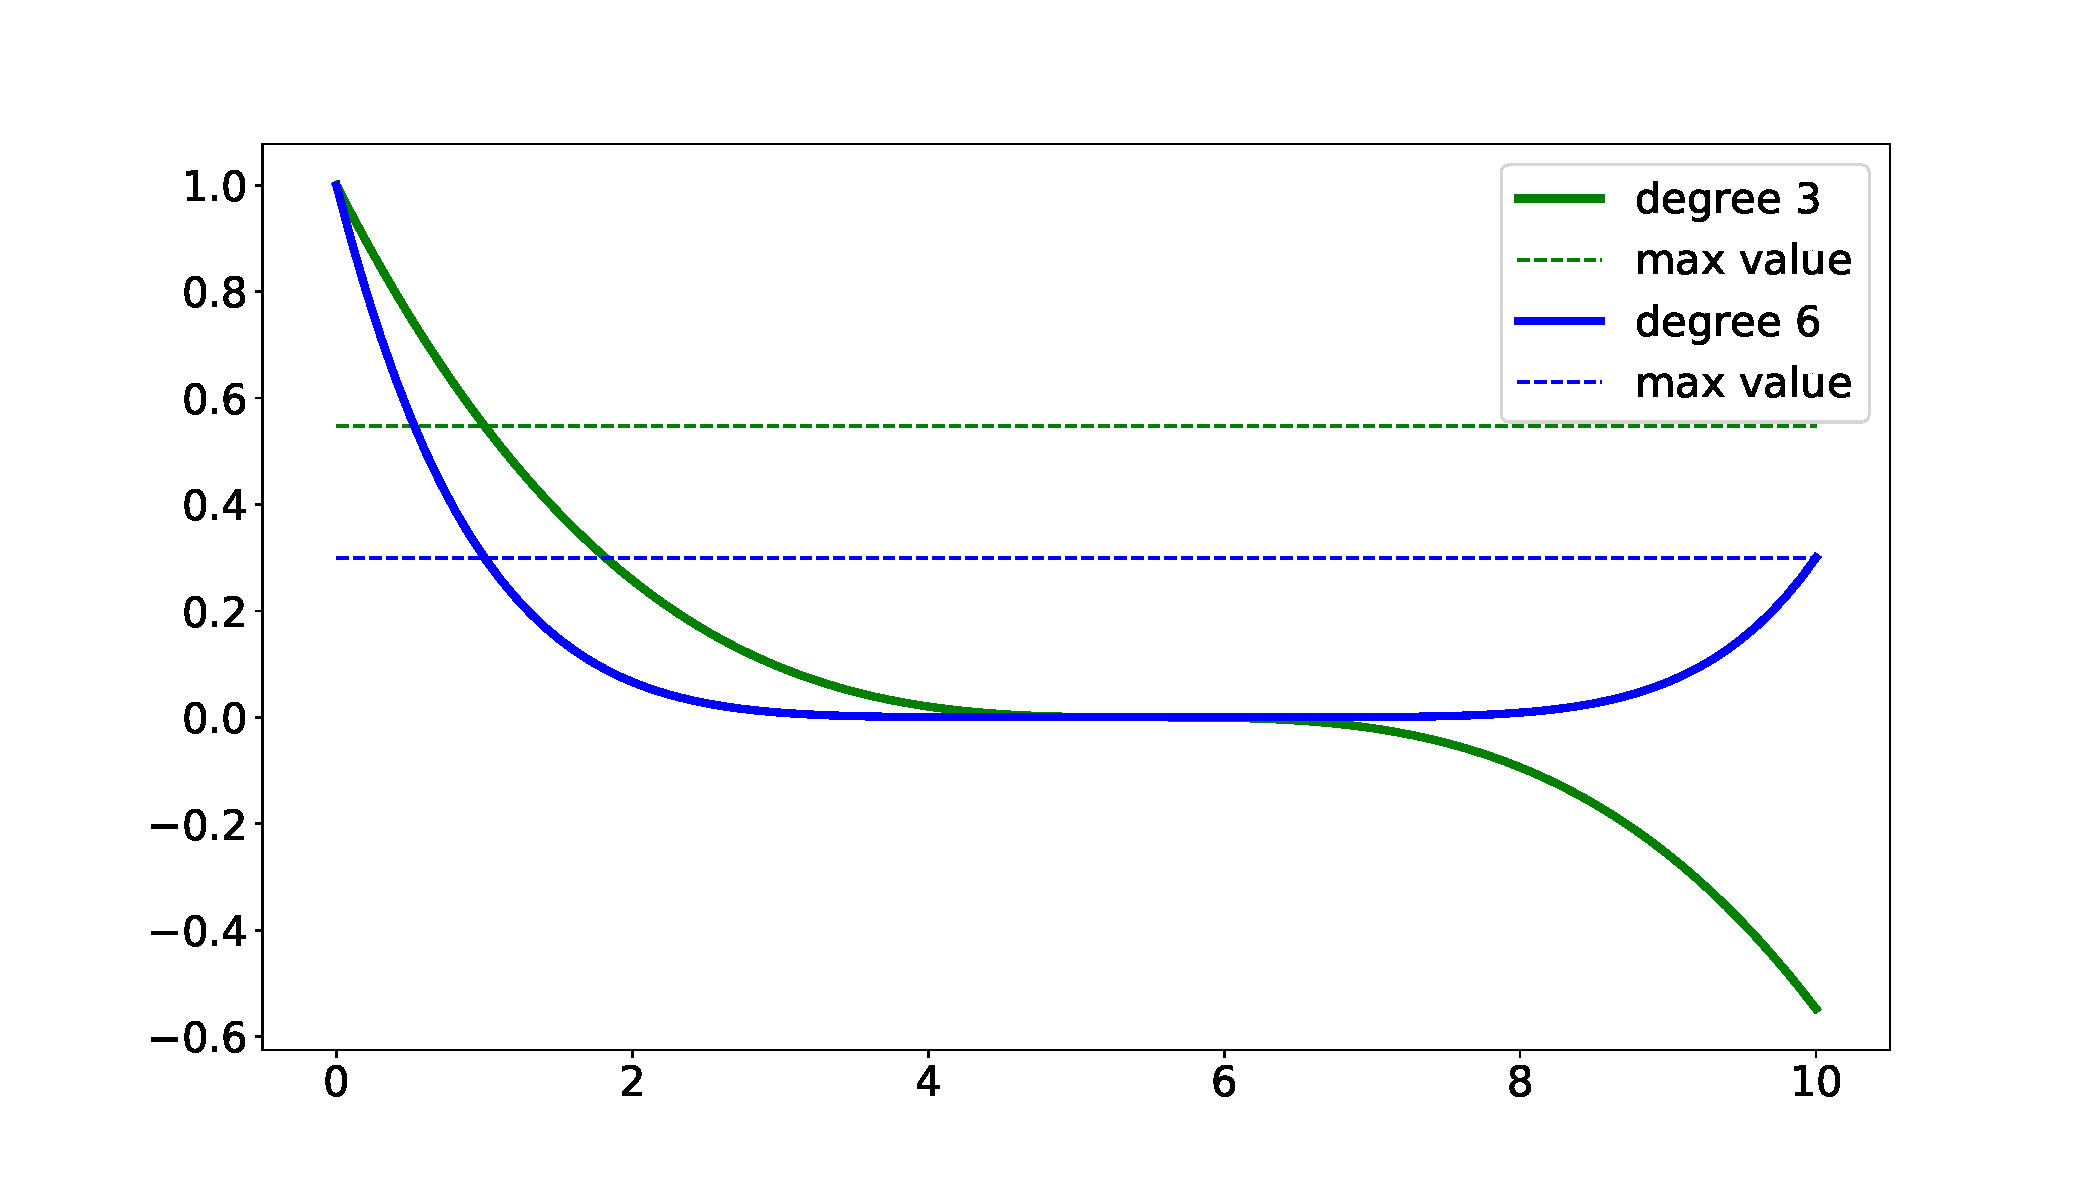
\includegraphics[width=0.9\textwidth]{figures/lecture6-naive_polynome.pdf}
\centering
\caption{Naive Polynomial}
\label{naive_p}
\end{figure}
%
The resulting polynomial $p_t(x)$ is plotted in Figure~\ref{naive_p} for degrees
$t = 3$ and $t = 6$, with $\alpha = 1$ and $\beta = 10$. Note that doubling the
degree from three to six only halves the maximum absolute value the polynomial
attains in $[\alpha,\beta]$, explaining why convergence is so slow.

\subsection{Chebyshev polynomials}
%
Fortunately, we can do better than this by speeding up gradient descent using
Chebyshev polynomials. We will use Chebyshev polynomials of the first kind,
defined by the recurrence relation:
\begin{align*}
T_0(a) &= 1,\quad T_1(a) = a \\
T_k(a) &= 2a T_{k-1}(a) - T_{k-2}(a),\ \text{for }k \geq 2\,.
\end{align*}
Figure \ref{chebychev_poly} plots the first few Chebyshev polynomials.

\begin{figure}[ht]
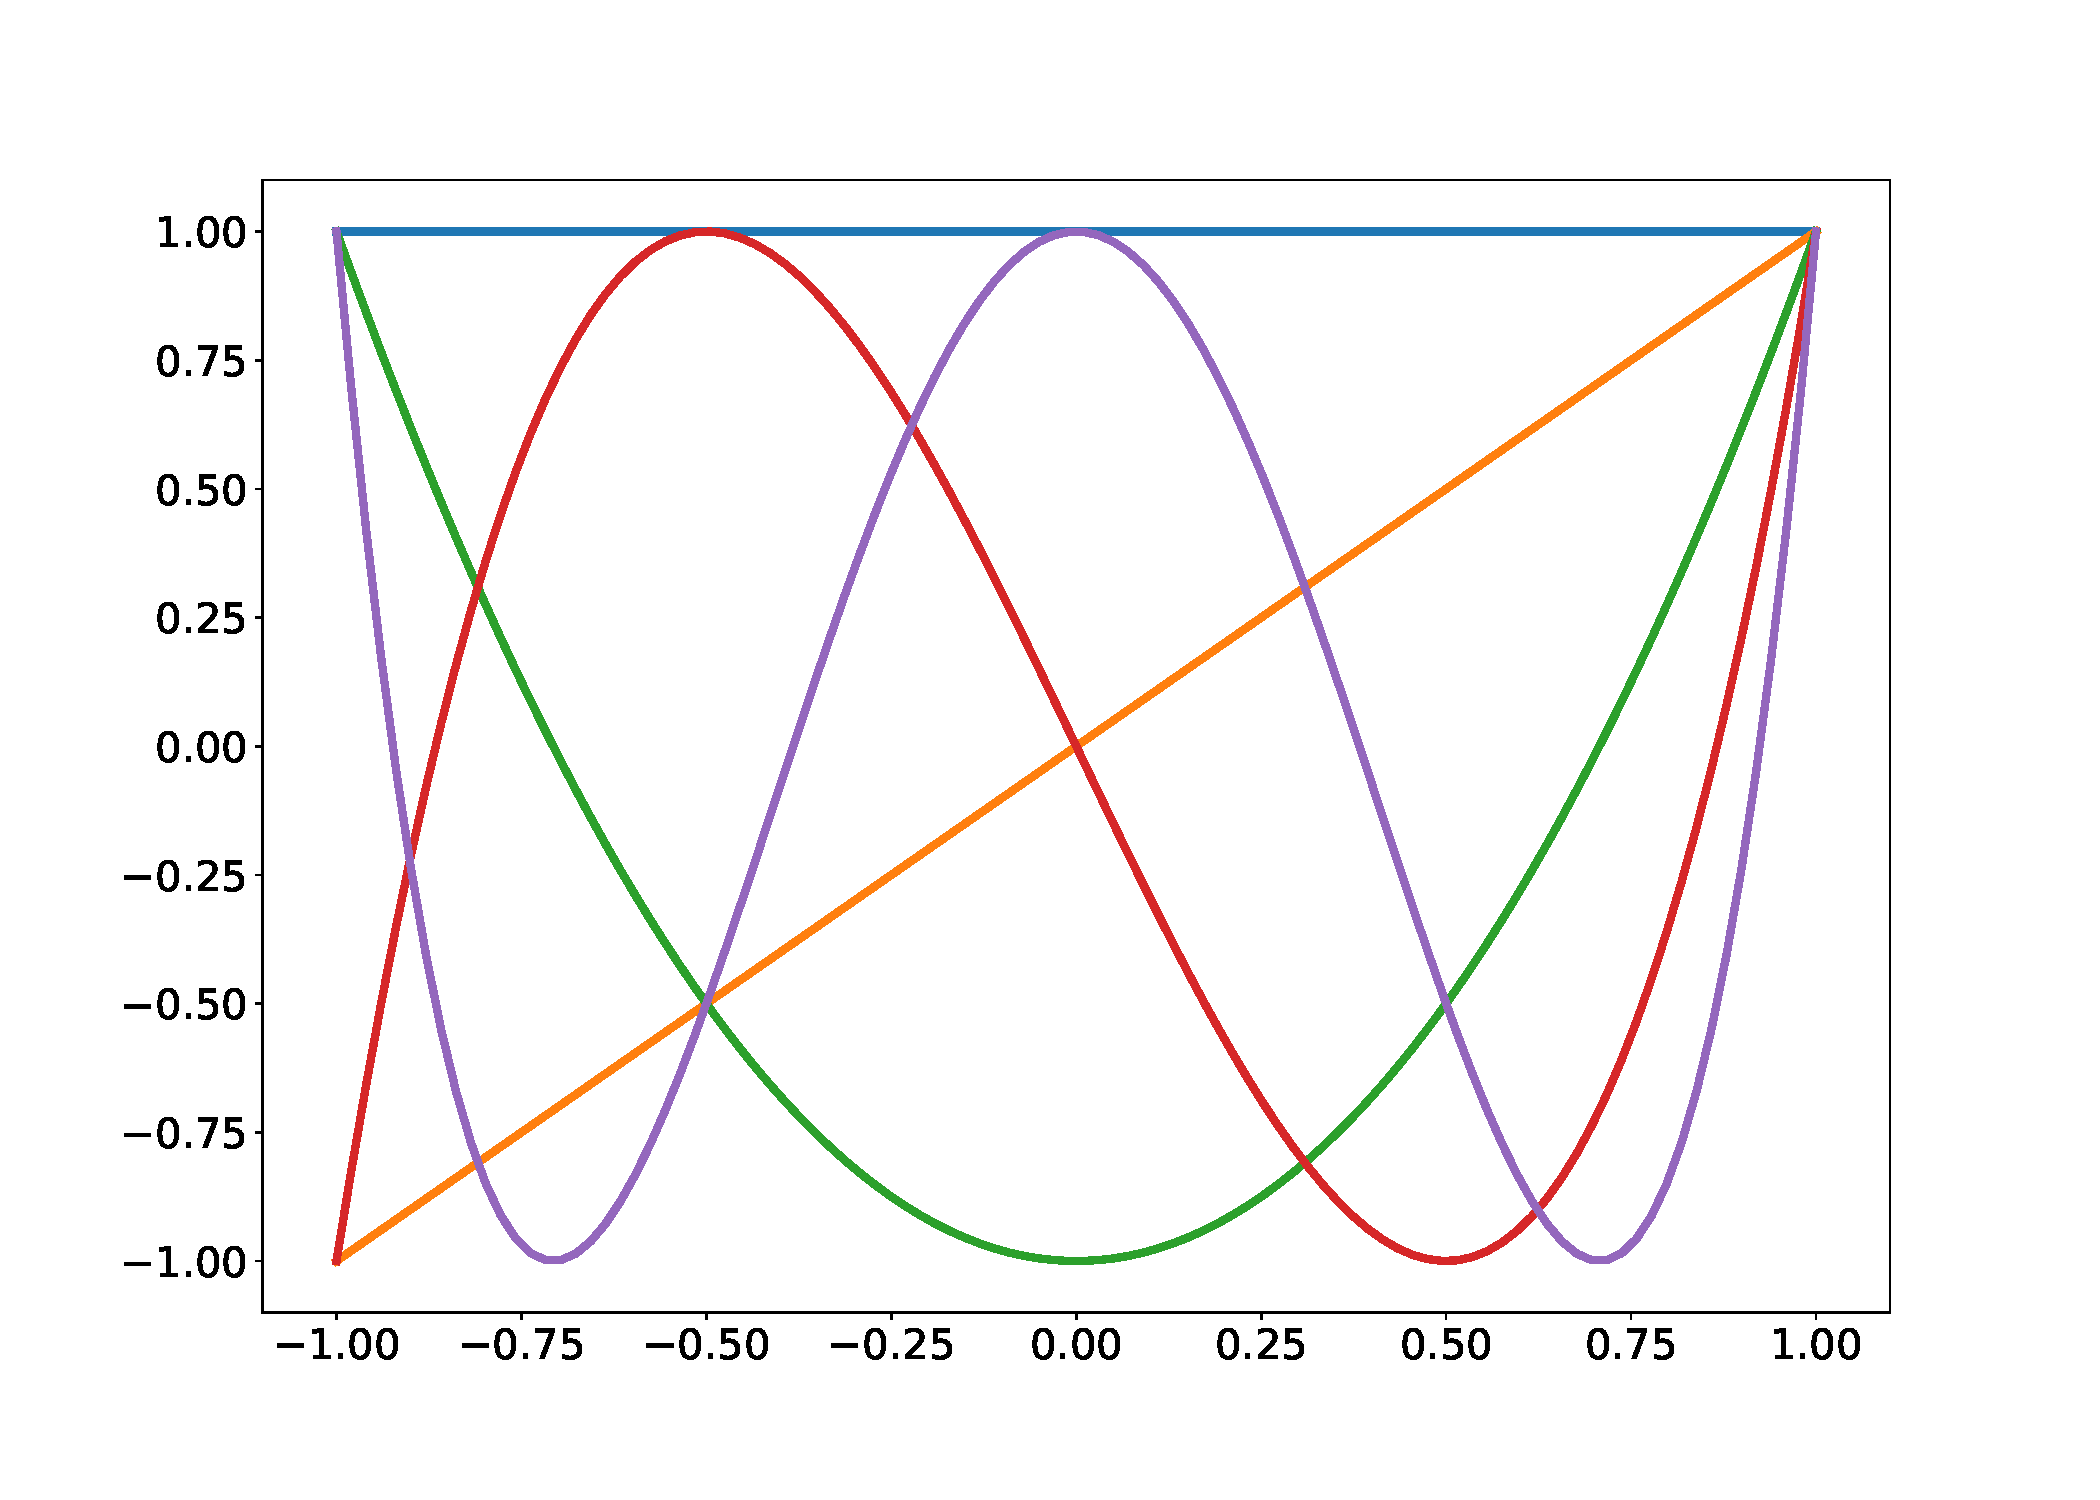
\includegraphics[width=0.9\textwidth]{figures/lecture6-cheb_polynome.pdf}
\centering
\caption{Chebychev polynomials of varying degrees.}
\label{chebychev_poly}
\end{figure}

Why Chebyshev polynomials? Suitably rescaled, they minimize the absolute value
in a desired interval $[\alpha, \beta]$ while satisfying the normalization
constraint of having value~$1$ at the origin.

Recall that the eigenvalues of the matrix we consider are in the interval $[\alpha, \beta]$. We need to rescale the Chebyshev polynomials so that they're supported on this interval and still attain value $1$ at the origin. This is accomplished by the polynomial

\begin{equation*}
P_k(a) = \frac{T_k\left(\frac{\alpha + \beta - 2a}{\beta - \alpha}\right)}{T_k\left(\frac{\alpha + \beta}{\beta - \alpha}\right)}.
\end{equation*}
\begin{figure}[ht]
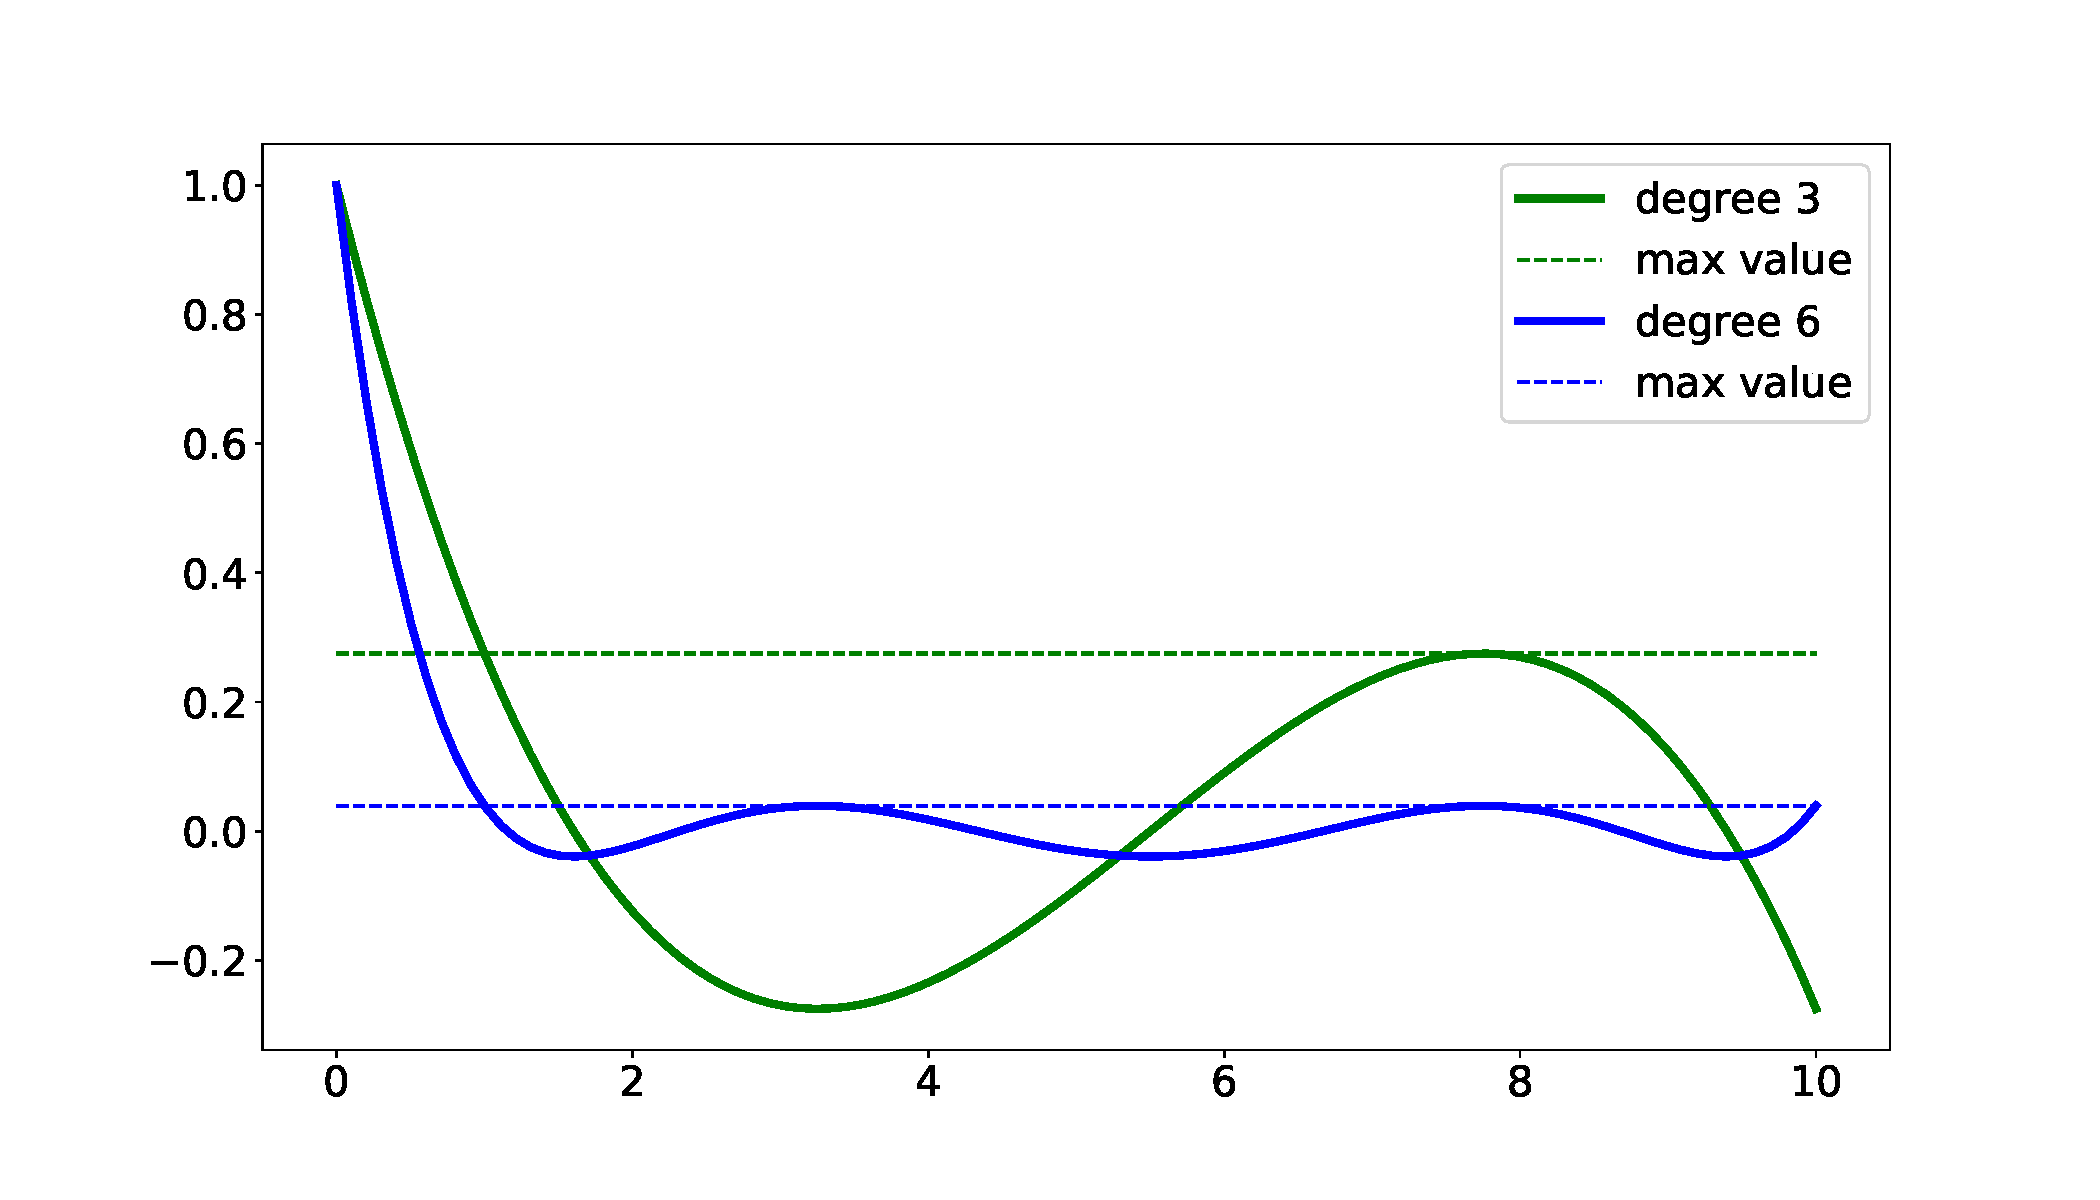
\includegraphics[width=0.9\textwidth]{figures/lecture6-rescaled_cheb.pdf}
\centering
\caption{Rescaled Chebyshev}
\label{rescales_chebyshev}
\end{figure}

\begin{figure}[ht]
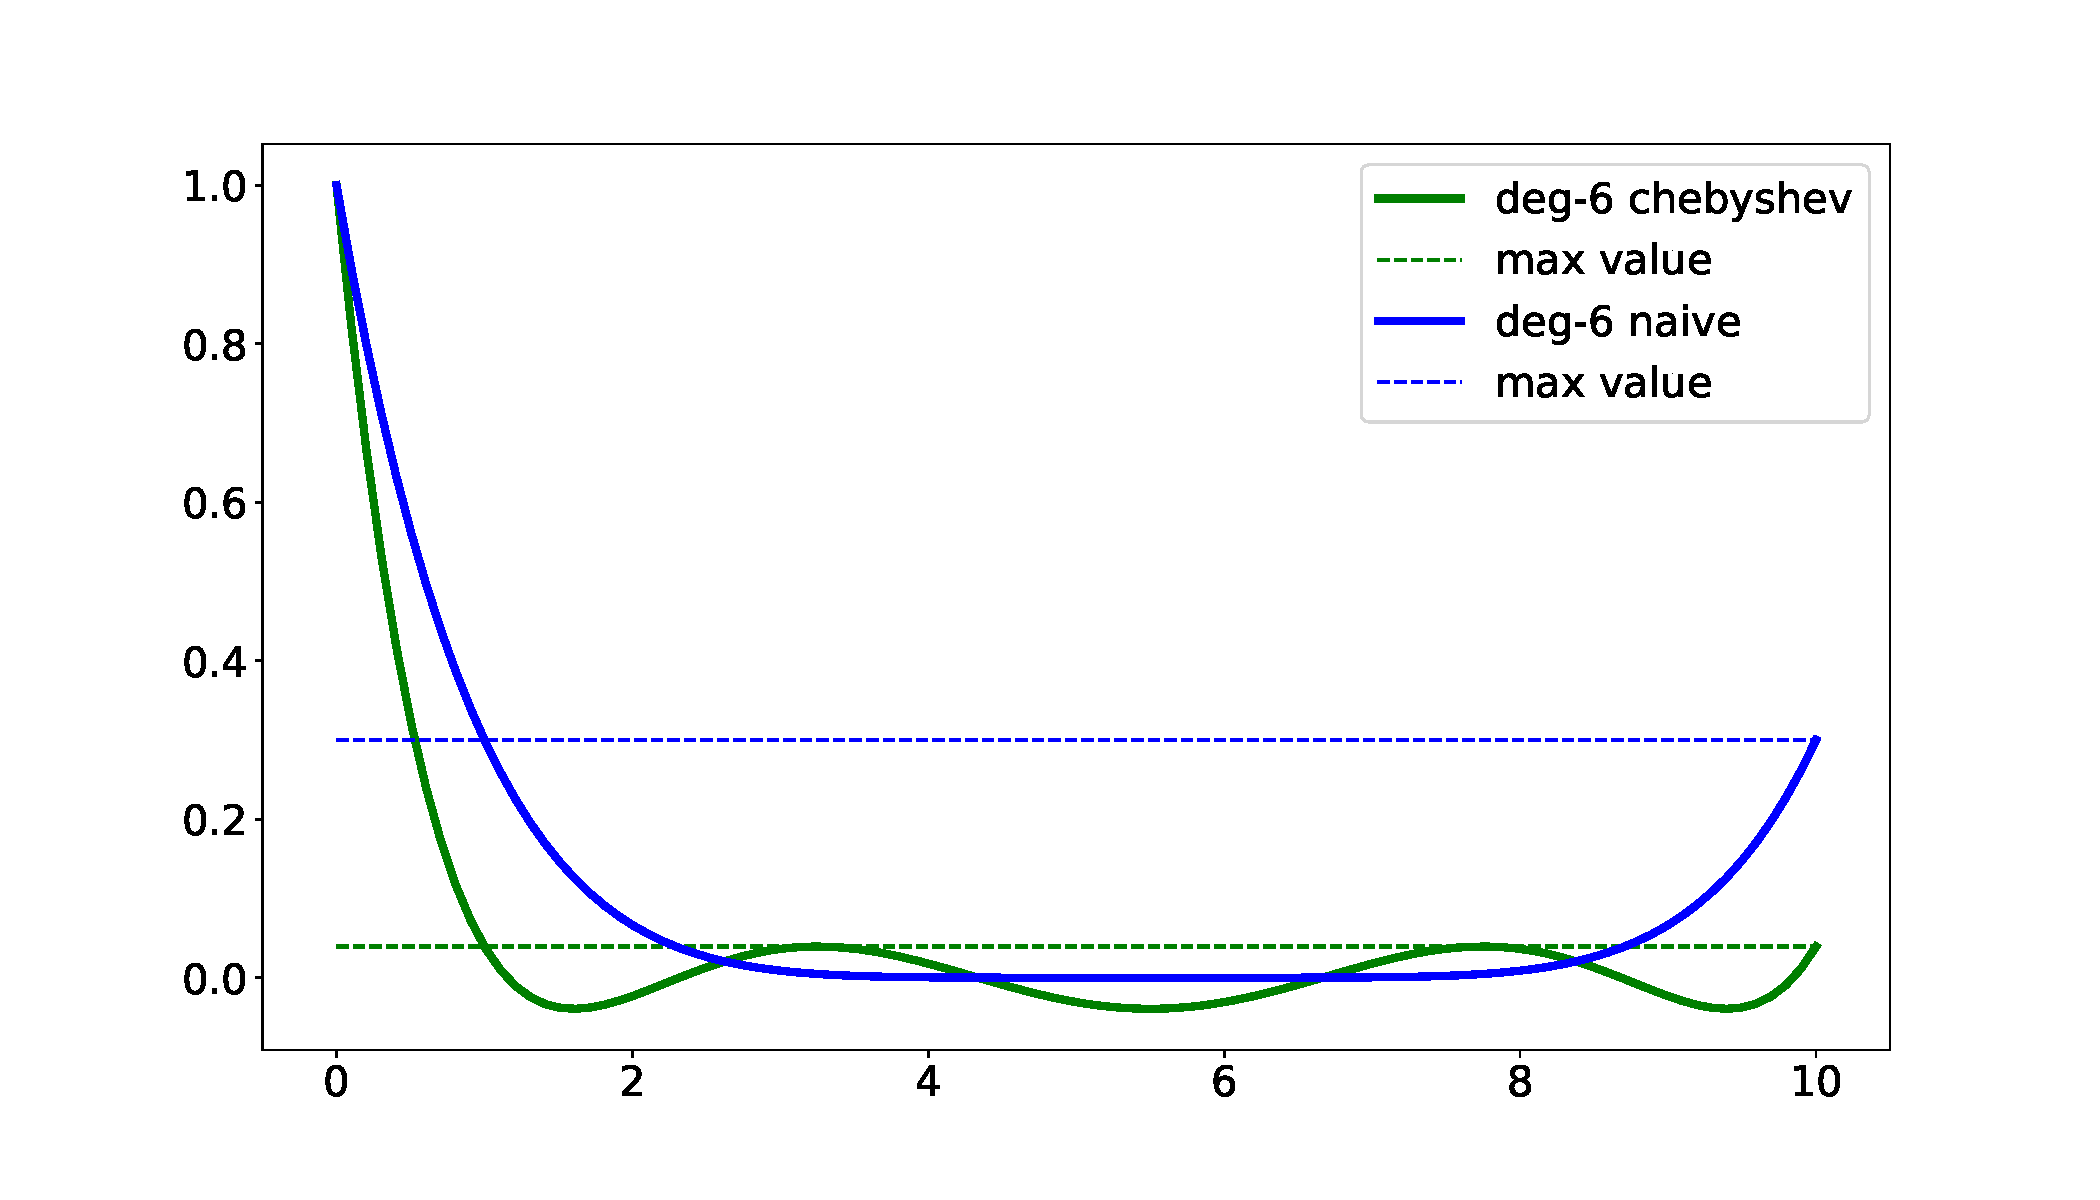
\includegraphics[width=0.9\textwidth]{figures/lecture6-rescaled_cheb_vs_naive.pdf}
\centering
\caption{Rescaled Chebyshev VS Naive Polynomial}
\label{rescaled_chebyshev_vs_naive_p}
\end{figure}

We see on figure \ref{rescales_chebyshev} that doubling the degree has a much more dramatic effect on the magnitude of the polynomial in the interval $[\alpha, \beta].$

Let's compare on figure \ref{rescaled_chebyshev_vs_naive_p} this beautiful Chebyshev polynomial side by side with the naive polynomial we saw earlier. The Chebyshev polynomial does much better: at around 0.3 for degree 3 (needed degree 6 with naive polynomial), and below 0.1 for degree 6.


\subsubsection{Accelerated gradient descent}

The Chebyshev polynomial leads to an accelerated version of gradient descent. Before we describe the iterative process, let's first see what error bound comes out of the Chebyshev polynomial.

So, just how large is the polynomial in the interval $[\alpha, \beta]$? First,
note that the maximum value is attained at $\alpha$. Plugging this into the
definition of the rescaled Chebyshev polynomial, we get the upper bound for any
$a\in[\alpha, \beta],$

\begin{align*}
|P_k(a)| &\leq |P_k(\alpha)| 
= \frac{|T_k(1)|}{|T_K\left(\frac{\beta + \alpha}{\beta - \alpha}\right)|} 
\le \left|T_K\left(\frac{\beta + \alpha}{\beta - \alpha}\right)^{-1}\right|.
\end{align*}
Recalling the condition number $\kappa=\beta/\alpha,$ we have
\begin{equation*}
\frac{\beta + \alpha}{\beta - \alpha} = \frac{\kappa + 1}{\kappa - 1}.
\end{equation*}
Typically $\kappa$ is large, so this is $1 + \epsilon$, $\epsilon \approx \frac{2}{\kappa}$. Therefore, we have
\begin{eqnarray*}
|P_k(a)| &\leq {|T_k(1 + \epsilon)^{-1}|}.
\end{eqnarray*}

To upper bound $|P_k|$, we need to lower bound $|T_k(1 + \epsilon)|$.

\textbf{Fact}: for $a > 1$, $T_k(a) = \cosh\left(k \cdot \mathrm{arccosh} (a)\right)$ where:
\begin{equation*}
\cosh(a) = \frac{e^a + e^{-a}}{2},\quad \mathrm{arccosh}(a) = \ln\left(x + \sqrt{x^2 - 1}\right).
\end{equation*}

Now, letting $\phi = \mathrm{arccosh}(1 + \epsilon)$:
\begin{equation*}
e^{\phi} = 1 + \epsilon + \sqrt{2\epsilon + \epsilon^2} \geq 1 + \sqrt{\epsilon}.
\end{equation*}
So, we can lower bound $|T_k(1 + \epsilon)|$:
\begin{align*}
|T_k(1 + \epsilon)| &= \cosh\left(k \mathrm{arccosh}(1 + \epsilon)\right) \\
&= \cosh(k\phi) \\
&= \frac{(e^\phi)^k + (e^{-\phi})^k}{2} \\
&\geq \frac{(1 + \sqrt{\epsilon})^k}{2}.
\end{align*}

Then, the reciprocal is what we needed to upper bound the error of our algorithm, so we have:
\begin{equation*}
|P_k(a)| \leq {|T_k(1 + \epsilon)^{-1}|} \leq 2(1 + \sqrt{\epsilon})^{-k}.
\end{equation*}

Thus, this establishes that the Chebyshev polynomial achieves the error bound:
\begin{align*}
\left\Vert x_{t+1} - x^* \right\Vert &\leq 2(1 + \sqrt{\epsilon})^{-t}
\left\Vert x_0 -x^*\right\Vert \\
&\approx 2\left(1 + \sqrt{\frac{2}{\kappa}}\right)^{-t} \left\Vert x_0 -x^*\right\Vert \\
&\leq 2\exp\left(-t \sqrt{\frac{2}{\kappa}}\right) \left\Vert x_0 -x^*\right\Vert.
\end{align*}

This means that for large $\kappa,$ we get quadratic savings in the degree we need before the error drops off exponentially. Figure \ref{convergence} shows the different rates of convergence, we clearly see that the 

\begin{figure}[ht]
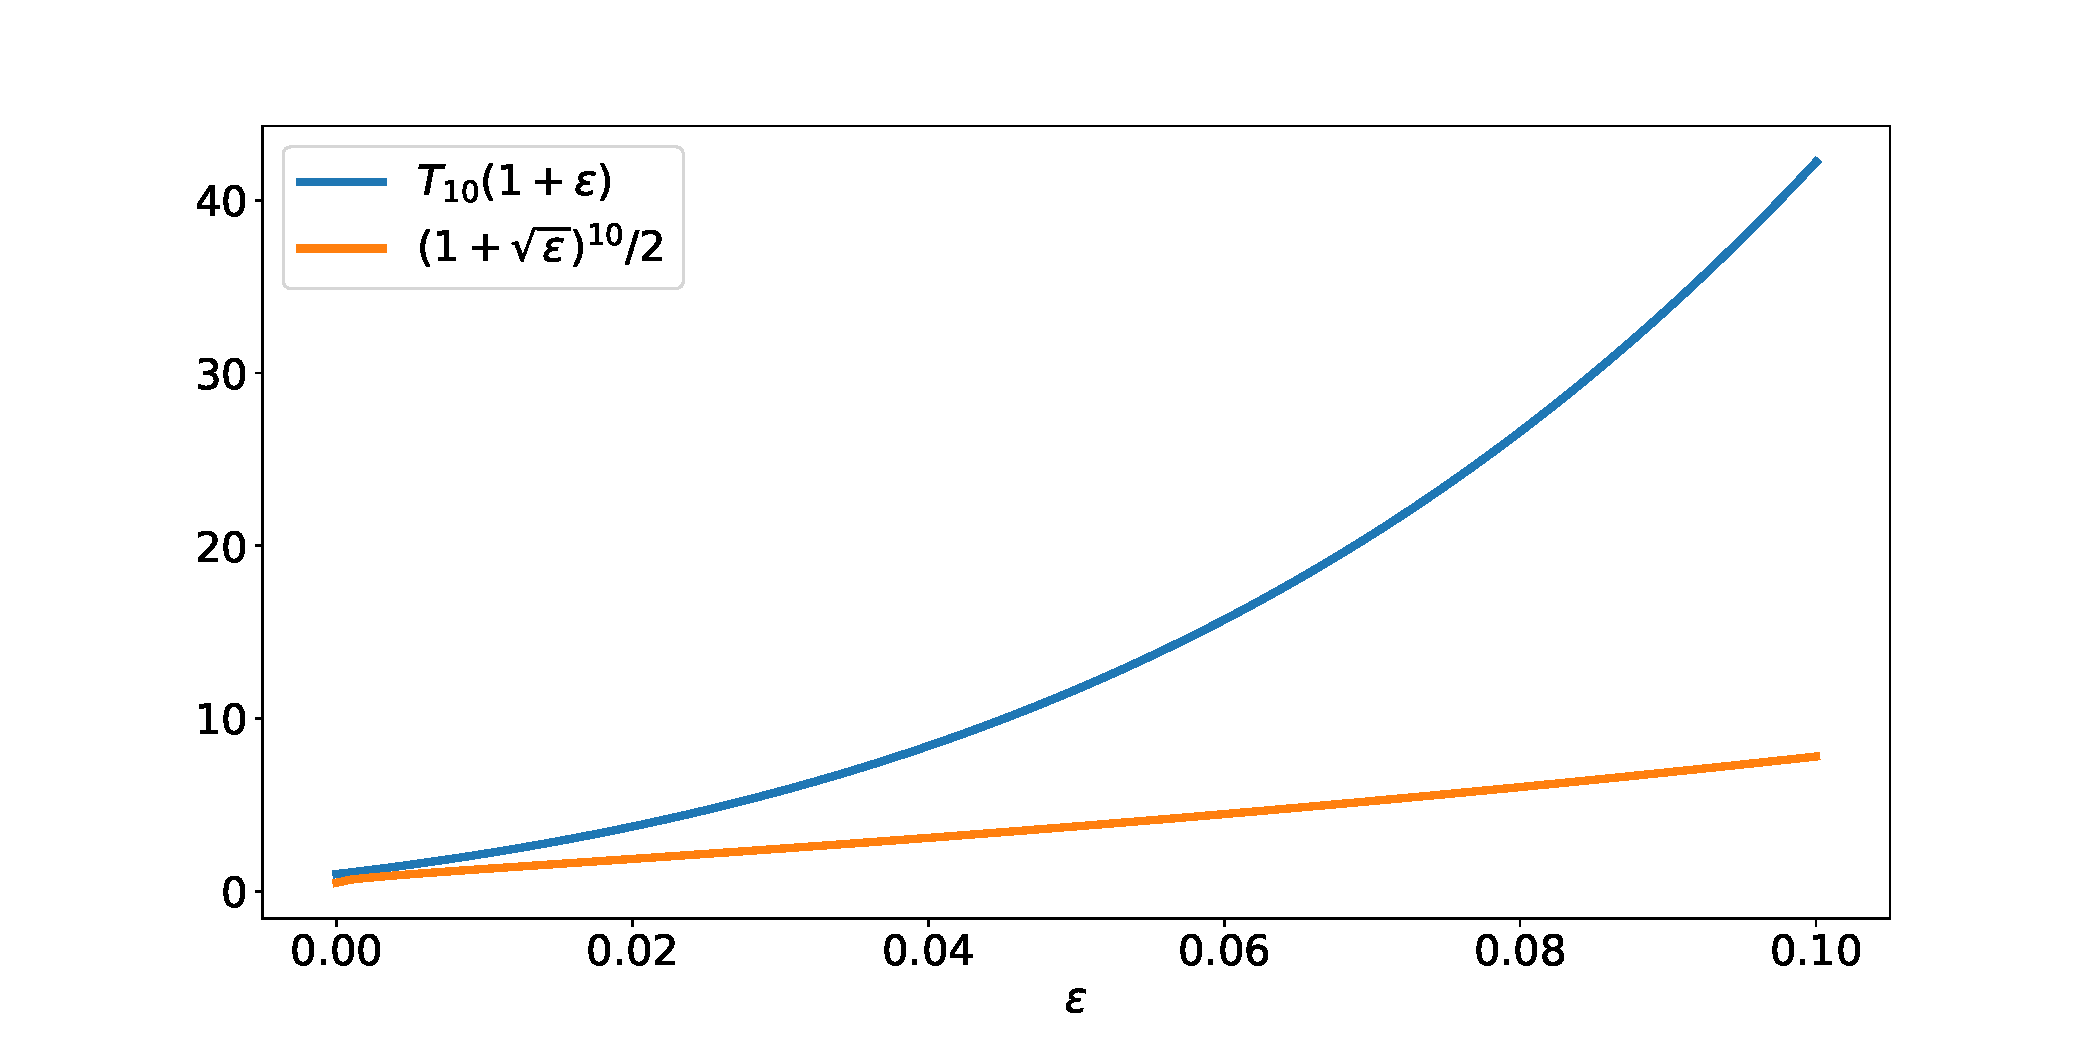
\includegraphics[width=0.9\textwidth]{figures/lecture6-conv.pdf}
\centering
\caption{Convergence for naive polynomial and Chebyshev}
\label{convergence}
\end{figure}

\subsubsection{The Chebyshev recurrence relation}
Due to the recursive definition of the Chebyshev polynomial, we directly get an iterative algorithm out of it. Transferring the recursive definition to our rescaled Chebyshev polynomial, we have:
\begin{equation*}
P_{K+1}(a) = (\eta_k a + \gamma_k)P_k(a) + \mu_k P_{k-1}(a).
\end{equation*}

where we can work out the coefficients $\eta_k,\gamma_k,\mu_k$ from the recurrence definition. Since $P_k(0)=1,$ we must have $\gamma_k+\mu_k=1.$ This leads to a simple update rule for our iterates:

\begin{eqnarray*}
x_{k+1} &= (\eta_k A + \gamma_k)x_k + (1 - \gamma_K)x_{k-1} - \eta_k b \\
&= (\eta_k A + (1 - \mu_k))x_k + \mu_k x_{k-1} - \eta_k b \\
&= x_k - \eta_k(Ax_k - b) + \mu_k(x_k - x_{k-1}).
\end{eqnarray*}

We see that the update rule above is actually very similar to plain gradient descent except for the additional term  $\mu_k(x_k - x_{k-1}).$ This term can be interpreted as a \textit{momentum} term, pushing the algorithm in the direction of where it was headed before. In the next lecture, we'll dig deeper into momentum and see how to generalize the result for quadratics to general convex functions.


\section{Lecture 7: Nesterov’s accelerated gradient descent}

Previously, we saw how we can accelerate gradient descent for minimizing
quadratics~$f(x)=x^\trans A x+b^\trans x,$ where $A$ is a positive definite
matrix. In particular, we achieved a quadratic improvement in the dependence
on the condition number of the matrix~$A$ than what standard gradient descent
achieved. The resulting update rule had the form
\[
x_{t+1} = x_t -\eta_t\nabla f(x_t) + \mu(x_t-x_{t-1})\,,
\]
where we interpreted the last term as a form of ``momentum''. In this simple
form, the update rule is sometimes called Polyak's \emph{heavy ball method}.

To get the same accelerated convergence rate for general smooth convex functions
that we saw for quadratics, we will have to work a bit harder and look into
Nesterov's celebrated \emph{accelerated gradient method}~\cite{Nesterov83,
Nesterov04}

Specifically, we will see that Nesterov's method achieves a convergence rate
of~$\cO \left(\frac{\beta}{t^2}\right)$ for $\beta$-smooth functions. For smooth
functions which are also $\alpha$-strongly convex, we will achieve a rate of
$\exp\left( -\Omega\left(\sqrt{\frac{\beta}{\alpha}} t\right)\right)$. 

The update rule is a bit more complicated than the plain momentum rule 
and proceeds as follows:
\begin{align*}
x_0 &= y_0 = z_0, \\
x_{t+1} &= \tau z_t + (1 - \tau) y_t \tag{$t\ge 0$}\\
y_t &= x_t - \frac{1}{\beta} \nabla f(x_t) \tag{$t\ge 1$}\\
z_t &= z_{t-1} - \eta\nabla f(x_t)\tag{$t\ge 1$}
\end{align*}
Here, the parameter~$\beta$ is the smoothness constant of the function we're
minimizing. The step size $\eta$ and the parameter~$\tau$ will be chosen below
so as to give us a convergence guarantee.

\subsection{Convergence analysis}

We first show that for a simple setting of the step sizes, the algorithm reduces
its initial error from some value~$d$ to $\frac{d}{2}.$ We will then repeatedly
restart the algorithm to continue reducing the error. This is a slight departure
from Nesterov's method which does not need restrating, albeit requiring a much
more delicate step size schedule that complicates the analysis.

\begin{lemma}
\lemmalabel{lecture7-main}
Suppose $f\colon\R^n\to\R$ is a convex, $\beta$-smooth function that attains its
minimum at a point~$x^*\in\R^n.$
Assume that the initial point satisfies $\|x_0-x^*\|\le R$ and $f(x_0)-f(x^*)\le
d.$ Put $\eta = \frac{R}{\sqrt{d\beta}}$, and 
$\tau$ s.t. $\frac{1-\tau}{\tau} = \eta \beta$.

Then after $T = 4R\sqrt{\frac{\beta}{d}}$ steps, 
we have 
\[
f(\bar{x})- f(x^*) \leq \frac{d}{2},
\]
where $\bar{x} = \frac{1}{T} \sum_{k=0}^{T-1} x_t$.
\end{lemma}

\begin{proof}
In Lecture~2, we showed the following properties for smooth and convex
functions:
\begin{equation}
\label{Nesterov-pf_smoothness_and_convexity}
f(y_t) - f(x_t) \leq -\frac{1}{2 \beta} \|\nabla f(x_t) \|^2
\end{equation}
By the ``Fundamental Theorem of Optimization" (see Lecture 2), we have
for all $u\in\R^n:$
\begin{align}
\label{lecture7-nonsmooth}
\eta\langle \nabla f(x_{t+1}), z_t - u \rangle 
&= \frac{\eta^2}2\|\nabla f(x_{t+1})\|^2 
+ \frac12\|z_t - u \|^2 - \frac12\|z_{t+1} - u \|^2\,.
\end{align}
Substituting the first equation yields
\begin{equation}
\eta \langle \nabla f(x_{t+1}, z_t - u \rangle \leq \eta^2 \beta (f(x_{t+1}) -
f(y_{t+1})) + \frac12\|z_t - u\|^2 - \frac12\|z_{t+1} - u \|^2 \label{Nesterov-pf_eq3}
\end{equation}
\medskip
Working towards a term that we can turn into a telescoping sum, we compute the
following difference
\begin{align}
&\eta \langle \nabla f(x_{t+1}), x_{t+1} - u\rangle - \eta \langle \nabla
f(x_{t+1}), z_t - u\rangle \nonumber\\
&= \eta \langle\nabla f(x_{t+1}), x_{t+1} - z_t\rangle \nonumber\\
&= \frac{1-\tau}{\tau}  \eta \langle\nabla f(x_{t+1}), y_t - x_{t+1}\rangle \nonumber\\
&\leq \frac{1-\tau}{\tau} \eta (f(y_t) - f(x_{t+1})) \quad\text{ (by convexity)}. \label{Nesterov-pf_eq4}
\end{align}
\medskip
Combining  \eqref{Nesterov-pf_eq3} and \eqref{Nesterov-pf_eq4}, and setting
$\frac{1-\tau}{\tau} = \eta \beta$ yield for all $u\in\R^n:$
\begin{equation*}
\eta\langle\nabla f(x_{t+1}), x_{t+1} - u\rangle \leq \eta^2 \beta
(f(y_t) - f(y_{t+1})) + \frac12\|z_t - u\|^2 - \frac12\|z_{t+1} - u\|^2.
\end{equation*}
Proceeding as in our basic gradient descent analysis, we apply this inequality
for $u=x^*,$ sum it up from $k=0$ to $T$ and exploit the telescoping effect:
\begin{align*}
\eta T (f(\bar{x}) - f(x^*)) 
&\leq \sum_{k=0}^T \eta \langle\nabla f(x_{t+1}), x_{t+1} - x^*\rangle\\
&\leq \eta^2 \beta d + R^2,
\end{align*}
which can be rewritten as
\begin{align*}
f(\bar{x}) - f(x^*) 
&\leq \frac{\eta\beta d}{T} + \frac{R^2}{\eta T} \\
&\leq \frac{2\sqrt{\beta d}}{T} R \tag{since $\eta=R/\sqrt{\beta d}$} \\
&\leq \frac{d}{2} \tag{since $T\ge 4R\sqrt{\beta/D}.$}
\end{align*}
\end{proof}

This lemma appears in work by Allen-Zhu and Orecchia~\cite{allen2014linear}, who
interpret Nesterov's method as a coupling of two ways of analyzing gradient
descent. One is the the inequality
in~\eqref{Nesterov-pf_smoothness_and_convexity} that is commonly used in the
analysis of gradient descent for smooth functions. The other is
Equation~\ref{lecture7-nonsmooth} commonly used in the convergence analysis for
non-smooth functions. Both were shown in our Lecture 2.

\begin{theorem}
\theoremlabel{lecture7-smooth}
Under the assumptions of \lemmaref{lecture7-main}, by restarting the algorithm
repeatedly, we can find a point $x$ such that
\[
f(x)-f(x^*)\le\epsilon
\]
with at most $O(R\sqrt{\beta/\epsilon})$ gradient updates.
\end{theorem}
\begin{proof}
By \lemmaref{lecture7-main}, we can go from error $d$ to $d/2$ with
$CR\sqrt{\beta/d}$ gradient updates for some constant~$C$. 
Initializing each run with the output of
the previous run, we can there for successively reduce the error from an initial
value~$d$ to $d/2$ to $d/4$ and so on until we reach error~$\epsilon$ after
$O(\log(d/\epsilon))$ runs of the algorithm. The total number of gradient steps
we make is
\[
CR\sqrt{\beta/d} 
+CR\sqrt{2\beta/d}
+\dots+CR\sqrt{\beta/\epsilon}
= O\left(R\sqrt{\beta/\epsilon}\right)\,.
\]
Note that the last run of the algorithm dominates the total number of steps up to a
constant factor.
\end{proof}

\subsection{Strongly convex case}

We can prove a variant of \lemmaref{lecture7-main} that applies when the
function is also $\alpha$-strongly convex, ultimately leading to a linear
convergence rate. The idea is just a general trick to convert a convergence rate
for a smooth function to a convergence rate in domain using the definition of
strong convexity.

\begin{lemma}
Under the assumption of \lemmaref{lecture7-main} and the additional assumption
that the function~$f$ is $\alpha$-strongly convex, we 
can find a point~$x$ with $T = O\left(\sqrt{\frac{\beta}{\alpha}}\right)$
gradient updates such that
\[
\|\bar x - x^*\|^2 \leq \frac12\|x_0-x^*\|^2\,.
\]
\end{lemma}
\begin{proof}
Noting that $\|x_0-x^*\|^2\le R^2,$ we can apply \theoremref{lecture7-smooth} with
error parameter $\epsilon = \frac{\alpha}4 \|x_0-x^*\|^2$ to find a point~$x$ such that
\[
f(x)-f(x^*)\le \frac\alpha4\|x_0-x^*\|^2\,,
\]
while only making $O\left(\sqrt{\beta/\alpha}\right)$ many steps.
From the definition of strong convexity it follows that
\[
\frac\alpha2 \|x-x^*\|^2 \le f(x)-f(x^*)\,.
\]
Combining the two inequalities gives the statement we needed to show.
\end{proof}

We see from the lemma that for strongly convex function we actually reduce the
distance to the optimum in domain by a constant factor at each step. We can
therefore repeatedly apply the lemma to get a linear convergence rate.

Table \ref{tab:nesterov} compares the bounds on error $\epsilon(t)$ as a
function of the total number of steps when applying Nesterov's method and
ordinary gradient descent method to different functions. 

\begin{table}[h]
  \begin{center}
    \begin{tabular}{ | l | c | c |}
      \hline
        & Nesterov's Method 
        & Ordinary GD Method \\ \hline
      $\beta$-smooth, convex 
      & \begin{tabular}{c}
        $O\left(\beta/t^2\right)$
        \end{tabular}
      & \begin{tabular}{c}
        $O\left(\beta/t\right)$
        \end{tabular} \\ \hline
      $\beta$-smooth, $\alpha$-strongly convex 
      & \begin{tabular}{c}
        $\exp\left(-\Omega(t\sqrt{\alpha/\beta})\right)$
        \end{tabular} 
      & \begin{tabular}{c}
        $\exp\left(-\Omega(t\alpha/\beta)\right)$
        \end{tabular} \\ \hline
    \end{tabular}
  \end{center}
  \caption{Bounds on error $\epsilon$ as a function of number of iterations $t$ for different methods.}
  \label{tab:nesterov}
\end{table}



\section{Lecture 8: Conjugate gradients and Krylov subspaces}
\sectionlabel{TBD}

In this lecture, we'll develop a unified view of solving linear equations~$Ax=b$
and eigenvalue problems~$Ax=\lambda x.$ In particular, we will justify the
following picture.
%
\begin{center}
\begin{tabular}{ | c |c| c | } 
\hline
 & $Ax=b$ & $Ax=\lambda x$ \\ 
\hline
Basic & Gradient descent & Power method \\ 
\hline
Accelerated & Chebyshev iteration & Chebyshev iteration \\
\hline
Accelerated and step size free & Conjugate gradient & Lanczos \\
\hline
\end{tabular}
\end{center}

What we saw last time was the basic gradient descent method and Chebyshev
iteration for solving quadratics. Chebyshev iteration requires step sizes to be
carefully chosen. In this section, we will see how we can get a ``step-size
free'' accelerated method, known as \emph{conjugate gradient}.

What ties this all together is the notion of a Krylov subspace and its
corresponding connection to low-degree polynomials.

Our exposition follows the excellent Chapter VI
in~Trefethen-Bau~\cite{trefethen97}.

\subsection{Krylov subspaces}
%
The methods we discuss all have the property that they generate a sequence of
points iteratively that is contained in a subspace called the \emph{Kyrlov
subspace}.
%
\begin{definition}[Krylov subspace]
For a matrix $A \in \R^{n x n}$ and a vector $b \in \R^n$, 
the \emph{Krylov sequence} of order $t$ is $b, Ab, A^2b, ...., A^tb$. 
We define the \emph{Krylov subspace} as
\[
K_t(A,b)=\mathrm{span}(\{b, Ab, A^2b, \ldots, A^t\}) \subseteq \R^n\,.
\]
\end{definition}

Krylov subspace naturally connect to polynomial approximation problems.
To see this, recall that a degree~$t$ matrix polynomial is an expression of the form
$p(A)=\sum_{i=1}^t \alpha_i A^i.$ 

\begin{fact}[Polynomial connection]
The Krylov subspace satisfies
\[
K_t(A,b) = \left\{ p(A)b : \text{deg}(p) \leq t \right\}\,.
\]
\end{fact}
\begin{proof}
Note that
\begin{align*}
v \in K_t(A,b) &\Longleftrightarrow \exists \alpha_i: \ v= \alpha_0 b + \alpha_1 Ab + \cdots \alpha_t A^tb
\end{align*}
\end{proof}


From here on, suppose we have a symmetric matrix $A \in \R^{n \times n}$ that
has orthonormal eigenvectors $u_1 \ldots u_n$ and ordered eigenvalues $\lambda_1
\geq \lambda_2 \ldots \geq \lambda_n$. Recall, this means
\begin{align*}
    \langle u_i,u_j\rangle &= 0,\quad\text{for } i \neq j\\
    \langle u_i, u_i\rangle &= 1 
\end{align*}
Using that $A=\sum_i \lambda_i u_i u_i^\trans,$ it follows
\[
p(A)u_i = p(\lambda_i)u_i\,.
\]
%
Now suppose we write $b$ in the eigenbasis of $A$ as 
\[
b=\alpha_1 u_1 + ... + \alpha_n u_n
\] 
with $\alpha_i = \langle u_i,b\rangle$. It follows that
\begin{align*}
p(A)b &= \alpha_1 p(\lambda_1)u_1 + \alpha_2 p(\lambda_2) u_2 + \ldots +
\alpha_n p(\lambda_n) u_n\,.
\end{align*}
 
\subsection{Finding eigenvectors}
Given these ideas, one natural approach to finding eigenvectors is to find a
polynomial~$p$ such that
\[
p(A)b \approx \alpha_1 u_1\,.
\]
Ideally, we would have $p(\lambda_1) = 1$ and $ p(\lambda_i) = 0$ for $i > 1$,
but this is in general impossible unless we maket he degree of our polynomial as
high as the number of distinct eigenvalues of~$A.$ Keep in mind that the degree
ultimately determines the number of steps that our iterative algorithm makes.
We'd therefore like to keep it as small as possible.

That's why we'll settle for an approximate solution that has $p(\lambda_1) = 1$
and makes $\max_{i > 1} p(\lambda_i)$ as small as possible. This will give us a close
approximation to the top eigenvalue. In practice, we don't know the
value~$\lambda_1$ ahead of time. What we therefore really care about is the
ratio $p(\lambda_1)/p(\lambda_2)$ so that no matter what~$\lambda_1,$ the second
eigenvalue will get mapped to a much smaller value by~$p.$ 

We consider the following simple polynomial~$p(\lambda)=\lambda^t$ that 
satisfies
\begin{align*}
    p(\lambda_2)/p(\lambda_1) &= \left(\frac{\lambda_2}{\lambda_1}\right)^t
\end{align*}
In the case where $\lambda_1=(1+\epsilon)\lambda_2$ we need $t=O(1/\epsilon)$ 
to make the ratio small.

The next lemma turns a small ratio into an approximation result for the
top eigenvector. To state the lemma, we recall that $\tan \angle (a,b)$ is the
tangent of the angle between $a$ and $b.$

\begin{lemma}
$\tan \angle(p(A)b, u_1) \leq \max_{j>1} \frac{|p(\lambda_j)|}{|p(\lambda_1)|}
\tan \angle (b, u_1)$
\end{lemma}

\begin{proof}
We define $\theta = \angle (u_1,b)$. By this, we get
\begin{align*}
    \sin ^2 \theta &=  \sum_{j >1} \alpha_j^2 \\
    \cos ^2 \theta &= |\alpha_1|^2 \\
    \tan^2 \theta &= \sum_{j > 1} \frac{|\alpha_j^2|}{|\alpha_1|^2}
\end{align*}
Now we can write:
\begin{align*}
    \tan^2 \angle (p(A)b, u_1) = \sum_{j>1}
\frac{|p(\lambda_j)\alpha_j|^2}{|p(\lambda_1)\alpha_1|^2} \leq
\underset{j>1}{\text{max}} \frac{|p(\lambda_j)|^2}{|p(\lambda_1)|^2} \sum_{j>1} \frac{\alpha_j |^2}{|\alpha_1| ^2}
\end{align*}
We note that this last sum $ \sum_{j > 1} \frac{\alpha_j |^2}{|\alpha_1| ^2}= \tan \theta$ and we obtain our desired result.
\end{proof}
Applying the lemma to $p(\lambda) = \lambda^t$ and $\lambda_1 =
(1+\epsilon) \lambda_2$, we get  
\[
\tan \angle(p(A)b, u_1) \leq
(1+\epsilon)^{-t} \tan \angle(u_1, b)\,.
\]
If there is a big gap between
$\lambda_1$ and $\lambda_2$ this converges quickly but it can be slow if
$\lambda_1 \approx \lambda_2$. It worth noting that if we choose $b\in\R^n$ to be a
random direction, then
\[
\E\left[\tan\angle(u_1,b)\right]=O\left(\sqrt{n}\right)\,.
\]
Going one step further we can also see that the expression $p(A)b=A^tb$ can of
course be built iteratively by repeatedly multiplying by~$A.$ For reasons of
numerical stability it makes sense to normalize after each matrix-vector
multiplication. This preserved the direction of the iterate and therefore does
not change our convergence analysis. The resulting algorithms is the well known
power method, defined recursively as follows:
%
\begin{align*}
x_0 &= \frac{b}{\|b\|} \\
x_t &= \frac{A x_{t-1}}{\|Ax_{t-1}\|}
\end{align*}
%
This method goes back more than hundred years to a paper by M\"untz in 1913, but
continues to find new applications today.
%
\subsection{Applying Chebyshev polynomials}

As we would expect from the development for quadratics, we can use Chebyshev
polynomials to get a better solution the polynomial approximation problem that
we posed above. The idea is exactly the same with the small difference that we
normalize our Chebyshev polynomial slightly differently.  This time around, we
want to ensure that $p(\lambda_1) = 1$ so that we are picking out the first
eigenvalue with the correct scaling. 

%\begin{tikzpicture}[scale = 0.8]
%  %\begin{axis}[doma
%  in= 2:8,xlabel=$\lambda$,label style={font=\large},tick label style={font=\large}, ylabel style={yshift=-.1cm}, xmin=0, xmax=13, ymin=-1, ymax=1.5, xtick={}, ytick={-1, 0,1},trig format plots=rad,grid=both,grid style={dashed,gray}]
%        \begin{axis}[%
%                width=10cm,
%                height=4cm,
%                scale only axis,
%                xmin=0, xmax=7,
%                xtick={0.5, 1, 1.5,2, 2.5,3, 3.5,4, 4.5, 5, 5.5, 5.75, 6,6.5},
%                xticklabels={$\lambda_n$,,,,,,,,,,,$\lambda_1$},
%                xmajorgrids,
%                ymin=-1, ymax=1.2,
%                ymajorgrids,
%                title={$p(0) = 1$},
%                axis lines*=left,
%                line width=1.0pt,
%                mark size=2.0pt,
%                legend style={at={(1.03,1)},anchor=north west,draw=black,fill=white,align=left}];
%                \addplot[domain = 0.5:5.75, black, very thick,samples=200] {.5*(cos(3*deg(x) ))};
%                \addplot[domain = 0:2] coordinates {(0,1)(0.5,0)};
%                \addplot[domain = 6.17:8.3] coordinates {(5.75,0)(6.45,1)};
%                \addplot[red] coordinates{(0.5,1)(0.5,-1)};
%                \addplot[red] coordinates{(5.75,1)(5.75,-1)};
%              
%               
%\end{axis}
%\end{tikzpicture}
%\begin{tikzpicture}[scale = 0.8]
%        \begin{axis}[%
%                width=10cm,
%                height=4cm,
%                scale only axis,
%                xmin=0, xmax=7,
%                xtick={0.5, 1, 1.5,2, 2.5,3, 3.5,4, 4.5, 5, 5.5, 6,6.5,7},
%                xticklabels={$\lambda_n$,,,,,,,,,,,,$\lambda_1$},
%                xmajorgrids,
%                ymin=-1, ymax=1.2,
%                ymajorgrids,
%                title={$p(\lambda_1) = 1$},
%                axis lines*=left,
%                line width=1.0pt,
%                mark size=2.0pt,
%                legend style={at={(1.03,1)},anchor=north west,draw=black,fill=white,align=left}];
%                \addplot[domain = 0.5:5.75, black, very thick,samples=200] {.5*(cos(3*deg(x) ))};
%                \addplot[domain = 0:2] coordinates {(0,1)(0.5,0)};
%                \addplot[domain = 6.17:8.3] coordinates {(5.75,0)(6.45,1)};
%                \addplot[red] coordinates{(0.5,1)(0.5,-1)};
%                \addplot[red] coordinates{(6.5,1)(6.5,-1)};
%              
%               
%\end{axis}
%\end{tikzpicture}

\begin{lemma}
A suitably rescaled degree $t$ Chebyshev polynomial achieves 
\begin{equation*}
\min_{p(\lambda_1)=1} \max_{\lambda \in [\lambda_2, \lambda_n]} p(\lambda) \leq
\frac{2}{(1+\max\{\sqrt{\epsilon},\epsilon\})^t}
\end{equation*}
where $\epsilon = \frac{\lambda_1}{\lambda_2} - 1$ quantifies the gap between the first
and second eigenvalue.
\end{lemma}

Note that the bound is much better than the previous one when~$\epsilon$ is
small. In the case of quadratics, the relevant ``$\epsilon$-value'' was the inverse
condition number. For eigenvalues, this turns into the gap between the first and
second eigenvalue.

\begin{center}
\begin{tabular}{ | c |c| c | } 
\hline
 & $Ax=b$ & $Ax=\lambda x$ \\ 
\hline
$\epsilon$ & $\frac{1}{\kappa} = \frac{\alpha}{\beta}$ & $\frac{\lambda_1}{\lambda_2} -1$ \\ 
\hline
\end{tabular}
\end{center}

As we saw before, Chebyshev polynomials satisfy a recurrence relation that can
be used to derive an iterative method achieving the bound above. The main
shortcoming of this method is that it needs information about the location of
the first and second eigenvalue. Instead of describing this algorithm, we move
on to an algorithm that works without any such information.

\subsection{Conjugate gradient method}
At this point, we switch back to linear equations~$Ax=b$ for a symmetric
positive definite matrix~$A\in\R^{n\times n}.$ The method we'll see is called
\emph{conjugate gradient} and is an important algorithm for solving linear
equations. Its eigenvalue analog is the Lanczos method. While the ideas behind
these methods are similar, the case of linear equations is a bit more intuitive.
%
\begin{definition}[Conjugate gradient method]
We want to solve $Ax = b,$ with  $A\succ 0$ symmetric. The conjugate gradient
method maintains a sequence of three points:
\begin{align*}
x_0 &= 0 \tag{ ``candidate solution''} \\
r_0 &= b \tag{ ``residual''} \\
p_0 &= r_0 \tag{ ``search direction''}
\end{align*}
For $t \ge 1:$
\begin{align*}
\eta_t &= \frac{\|r_t\|}{\langle p_{t-1}, Ap_{t-1}\rangle} \tag{``step size''} \\
x_t &= x_{t-1} + \eta_t p_{t-1} \\
r_t &= r_{t-1} - \eta_t A r_{t-1} \\
p_t &= r_t + \frac{\|r_t\|^2}{\|r_{t-1}\|^2}p_{t-1}
\end{align*}
\end{definition}

\begin{lemma}
\lemmalabel{lecture8-conjugategradient}
The following three equations must always be true for the conjugate gradient
method algorithm:
\begin{itemize}
\item $\mathrm{span}(\{r_0, ...r_{t-1}\}) = K_t(A,b)$
\item For $j<t$ we have $\langle r_t, r_j\rangle = 0$ and in particular
$r_t \perp K_t(A,b).$
\item The search directions are conjugate $p_i^{\trans} A p_j = 0$ for $i\ne j.$
\end{itemize}
\end{lemma}
\begin{proof}
Proof by induction (see Trefethen and Bau). Show that the conditions are true
initially and stay true when the update rule is applied.  
\end{proof}

\begin{lemma}
Let $\|u\|_A = \sqrt{u^\trans A u}$ and $\langle u,v\rangle_A = u^\trans A v$ and 
$e_t = x^* - x_t$. Then $e_t$ minimizes $\|x^* - x\|_A$ over all vectors $x \in K_{t-1}$.
\end{lemma}

\begin{proof}
We know that $x_t \in K_t$. Let $x \in K_t$ and define $x = x_t - \delta$. 
Then, $e = x^* - x = e_t + \delta.$
We compute the error in the $A$ norm:
\begin{align*}
\|x^* - x\|_A^2 
&= (e_t + \delta)^{\trans} A(e_t + \delta) \\
&= e_t^{\trans}Ae_t + \delta^{\trans}A\delta + 2e_t^{\trans} A \delta\,
\end{align*}
Bby definition~$e_t^{\trans}A = r_t$.
Note that $\delta \in K_t.$ 
By \lemmaref{lecture8-conjugategradient}, we have that $r_t \perp K_t(A,b).$
Therefore, $2e_t^{\trans} A \delta = 0$ and hence, 
\begin{align*}
\|e\|_A^2
= \|x^* - x\|_A^2 
= e_t^{\trans}Ae_t + \delta^{\trans}A\delta
\ge \|e_t\|_A\,.
\end{align*}
In the last step we used that $A\succ0.$
\end{proof}

What the lemma shows, in essence, is that conjugate gradient solves the
polynomial approximation problem:
\[
\min_{p\colon\deg(p)\le t, p(0)=1} \|p(A)e_0\|_A\,.
\]
Moreover, it's not hard to show that
\[
\min_{p\colon\deg(p)\le t, p(0)=1} 
\frac{\|p(A)e_0\|_A}{\|e_0\|_A}
\le 
\min_{p\colon\deg(p)\le t, p(0)=1} 
\max_{\lambda\in\Lambda(A)}\left| p(\lambda)\right|\,.
\]
In other words, the error achieved by conjugate gradient is no worse that the
error of the polynomial approximation on the RHS, which was solved by the
Chebyshev approximation. From here it follows that conjugate gradient must
converge at least as fast in $\|\cdot\|_A$-norm than Chebyshev iteration.


\section{Lower bounds and trade-offs}

\emph{Coming soon}

\part{Stochastic optimization}
\section{Lecture 10: Stochastic optimization}
The goal in stochastic optimization is to 
minimize functions of the form
\[
    f(x) = \E_{z\sim \cD}g(x,z)\,
\]
which have stochastic component given by a distribution~$\cD.$ In the case where
the distribution has finite support, the function can be written as
\[
    f(x) = \frac{1}{m}\sum_{i=1}^m f_i(x)\,.
\]
To solve these kinds of problems, we examine the stochastic gradient descent
method and some if its many applications.

\subsection{The stochastic gradient method}

Following Robbins-Monro \cite{Robbins&Monro:1951}, we define the stochastic
gradient method as follows. 

\begin{definition}[Stochastic gradient method]
The stochastic gradient method starts from a point $x_0\in\domain$ and proceeds
according to the update rule
\begin{equation*}
    x_{t+1} = x_t - \eta_t\nabla f_{i_t}(x_t) 
\end{equation*}
where $i_t\in\{1,\dots,m\}$ is either selected at random at each step, or cycled
through a random permutation of $\{1,\dots,m\}$.
\end{definition}

Either of the two methods for selecting~$i_t$ above, lead to the fact that
\[
    \E\nabla f_{i_t}(x) = \nabla f(x)
\]
This is also true when $f(x)=\E g(x,z)$ and at each step we update according to
$\nabla g(x,z)$ for randomly drawn~$z\sim\cD.$
%
\subsubsection{Sanity check}

Let us check that on a simple problem that the stochastic gradient descent yields the optimum. Let $p_1, \dots, p_m\in \R^n$, and define $f\colon \R^n \rightarrow \R_+$:
\begin{equation*}
    \forall x\in \R^n,\ f(x) = \frac{1}{2m}\sum_{i=1}^m \|x-p_i\|_2^2
\end{equation*}
Note that 
here $f_i(x) = \frac{1}{2}\|x-p_i\|_2^2$ 
and $\nabla f_i(x) = x-p_i.$ 
Moreover,
\begin{equation*}
    x^* = \argmin_{x\in\R^d} f(x) = \frac{1}{m}\sum_{i=1}^mp_i
\end{equation*}

Now, run SGM with $\eta_t=\frac{1}{t}$ in cyclic order i.e. $i_t = t$ and $x_0=0$:
\begin{align*}
    x_0 &= 0 \\
    x_1 &= 0 - \frac{1}{1}(0-p_1) = p_1 \\
    x_2 &= p_1 - \frac{1}{2}(p_1-p_2) = \frac{p_1+p_2}{2}\\
    \vdots\\
    x_n &= \frac{1}{m}\sum_{i=1}^mp_i = x^*
\end{align*}

\subsection{The Perceptron}

The
\href{https://www.nytimes.com/1958/07/08/archives/new-navy-device-learns-by-doing-psychologist-shows-embryo-of.html}{New
York Times} wrote in 1958 that the Perceptron \cite{Rosenblatt58theperceptron:}
was:
\begin{quote}
\emph{the embryo of an electronic computer that [the Navy] expects will be able
to walk, talk, see, write, reproduce itself and be conscious of its existence.}
\end{quote}

So, let's see.

\begin{definition}[Perceptron] 
Given labeled points~$((x_1, y_1),\dots,(x_m,y_m))\in(\R^n\times\{-1,1\})^m,$ 
and and initial point~$w_0\in\R^n$, the Perceptron is the following algorithm. 
For $i_t\in\{1,\dots,m\}$ selected uniformly at random,
\begin{equation*}
w_{t+1} =w_t(1-\gamma) + \eta \begin{cases}
    y_{i_t}x_{i_t}& \text{if } y_{i_t}\langle w_t, x_{i_t}\rangle <1\\
    0              & \text{otherwise}
\end{cases}
\end{equation*}
\end{definition}

Reverse-engineering the algorithm, the Perceptron is equivalent to running the
SGM on the Support Vector Machine (SVM) objective function.

\begin{definition}[SVM] 

Given labeled points~$((x_1, y_1),\dots,(x_m,y_m))\in(\R^n\times\{-1,1\})^m,$ 
the SVM objective function is:
\begin{equation*}
    f(w) = \frac{1}{n}\sum_{i=1}^m \max(1-y_i\langle w, x_i\rangle,\; 0) + \lambda \|w\|_2^2
\end{equation*}
The loss function $\max(1-z,\;0)$ is known as the Hinge Loss. The extra 
term~$\lambda \|w\|_2^2$ is known as the regularization term.
\end{definition}

\subsection{Empirical risk minimization}
We have two spaces of objects $\mathcal{X}$ and ${\mathcal{Y}},$ where we think
of $\mathcal{X}$ as the space of \emph{instances} or \emph{examples}, and
$\mathcal{Y}$ is a the set of \emph{labels} or \emph{classes}.

Our goal is to \emph{learn} a function $h\colon\mathcal{X}\to\mathcal{Y}$ which
outputs an object $y\in \mathcal{Y}$, given $ x\in \mathcal{X}$.  Assume there
is a joint distribution $\mathcal{D}$ over the space~$\mathcal{X} \times
\mathcal{Y}$ and the training set consists of $m$ instances $(x_1, y_1), \ldots,
(x_m,y_m)$ drawn i.i.d.~from $\mathcal{D}$.

We also define a non-negative real-valued loss function $\ell(y^\prime,y)$ to
measure the difference between the prediction $y^\prime$ and the true outcome
$y$.

\begin{definition}
The risk associated with h(x) is defined as the expectation of the loss function:
\begin{equation*}
    R[h] = \mathbb{E}_{\mathcal{X} \times \mathcal{Y} \in \mathcal{D}} \ell(h(x),y)
\end{equation*}
\end{definition}
The ultimate goal of a learning algorithm is to find $h^*$ among a class of functions $\mathcal{H}$ that minimizes $R[h]$:
\begin{equation*}
    h^* = \text{arg}\min_{h \in \mathcal{H}} R[h]
\end{equation*}
In general, the risk $R[h]$ can not be computed because the joint distribution is unknown. Therefore,

The \emph{empirical risk} is defined by averaging the loss function of the training set:
\begin{equation*}
    R_n[h] = \frac{1}{n} \sum^n_{i=1}\ell(h(x_i),y_i)
\end{equation*}
An empirical risk minimizer is any point $h^* \in \arg\min_{h \in \mathcal{H}} R_n[h]$.

The stochastic gradient method can be thought of as minimizing the risk
directly, if each example is only used once. In cases where we make multiple
passes over the training set, it is better to think of it as minimizing the
empirical risk, which can give different solutions than minimizing the risk.
We'll develop tools to relate risk and empirical risk in the next lecture.

\subsection{Online Learning}

An interesting variant of this learning setup is called \emph{online learning}.
It arises when we do not have a set of training data, but rather must make
decisions one-by-one.

\paragraph{Taking advice from experts.}
Imagine we have access to the predictions of $n$ experts. 
We start from an initial distribution over experts, given by
weights~$w_1\in\Delta_n = \{ w\in\R^n\colon \sum_i w_i=1, w_i\ge0\}.$

At each step $t = 1, \ldots, T$:
\begin{itemize}
    \item we randomly choose an expert according to~$w_t$
    \item nature deals us a loss function $f_t\in[-1,1]^n,$ specifying for each
expert~$i$ the loss~$f_t[i]$ incurred by the prediction of expert~$i$ at
time~$t.$
    \item we incur the expected loss $\E_{i\sim w_t}f_t[i]=\langle
w_t,f_t\rangle.$
    \item we get to update our distribution to from $w_t$ to $w_{t+1}.$
\end{itemize}

At the end of the day, we measure how well we performed relative to the best
fixed distribution over experts in hindsight. This is called \emph{regret}:
\begin{equation*}
   R = \sum^T_{t = 1} \langle w_{t}, f_t \rangle - \min_{w \in \Delta_n} \sum^{T}_{t = 1} \langle w, f_t \rangle
\end{equation*}
This is a relative benchmark. Small regret does not say that the loss is necessarily
small. It only says that had we played the same strategy at all steps, we
couldn't have done much better even with the benefit of hindsight.

\subsection{Multiplicative weights update}

Perhaps the most important online learning algorithm is the \emph{multiplicative
weights update}. Starting from the uniform distribution~$w_1,$ proceed according
to the following simple update rule for $t>1,$
\begin{align*}
    v_t[i] &= w_{t-1}[i]e^{-\eta f_t[i]} \tag{exponential weights update}\\
    w_t &= v_t/(\textstyle\sum_i v_t[i]) \tag{normalize}
\end{align*}
The question is \textit{how do we bound the regret} of the multiplicative
weights update? We could do a direct analysis, but instead we'll relate
multiplicative weights to gradient descent and use the convergence guarantees
we already know.

\subsection{Multiplicative weights as mirror descent}

Recall that mirror descent requires a mirror map $\phi : \Omega \to R$ over a
domain $\Omega \in \mathbb{R}^n$ where $\phi$ is strongly convex and
continuously differentiable.

The associated projection is
\begin{equation*}
    \Pi^\phi_\domain (y) = \argmin_{x\in\domain} \mathcal{D}_\phi(x,y)
\end{equation*}
where $\mathcal{D}_\phi(x,y)$ is Bregman divergence.
\begin{definition}
The Bregman divergence measures how good the first order approximation of the
function~$\phi$ is:
    \begin{equation*}
        \mathcal{D}_\phi(x,y) = \phi(x) - \phi(y) - \nabla \phi(y) ^\intercal (x-y)
    \end{equation*}
\end{definition}
The mirror descent update rule is:
\begin{align*}
    \nabla \phi(y_{t+1}) &= \nabla \phi (x_t) - \eta g_t \\
    x_{t+1} &=  \Pi^\phi_\domain (y_{t+1})
\end{align*}
where $g_t \in \partial f(x_t).$ 
In the first homework, we proved the following results.
\begin{theorem}
    let $\|\cdot\|$ be arbitrary norm and suppose that $\phi$ is $\alpha$-strongly convex      \textbf{w.r.t.} $\|\cdot\|$ on $\domain$. Suppose that $f_t$ is $L$-lipschitz \textbf{w.r.t.} $\|\cdot\|$, we have:
    \begin{equation*}
        \frac{1}{T}\sum^T_{t=1} f_t(x_t) \leq \frac{ \mathcal{D}_\phi(x^*,x_0)}{T \eta}+ \eta \frac{L^2}{2\alpha}
    \end{equation*}
\end{theorem}


Multiplicative weights are an instance of the Mirror Descent where $\Phi(w)=
\sum_{i=1}^m w_i \log(w_i)$ is the negative entropy function.
We have that
\[
\nabla\Phi(w) =  1 + \log(w),
\]
where the logarithm is elementwise.
The update rule in Mirror Descent becomes:
\begin{align*}
    \nabla\Phi(v_{t+1}) &=\nabla\Phi(w_{t}) - \eta_tf_t \\
    \implies v_{t+1} &= w_te^{-\eta_t f_t}
\end{align*}

Now comes the projection step. The Bregman divergence is, for all $(x,y)\in\domain^2$:
\begin{align*}
    D_{\Phi}(x,y) &= \Phi(x)-\Phi(y) - \nabla\Phi(y)^T(x-y)\,.
\end{align*}
If we write out this expression and simplify, we recover the well-known
\emph{relative entropy}. The projection
\begin{align*}
    \Pi_{\domain}^{\Phi}(y) = \argmin_{x\in\domain}D_{\Phi}(x,y)
\end{align*}
turns out to just correspond to the normalization step in the update rule.

\paragraph{Concrete rate of convergence.}
To get a concrete rate of convergence from the preceeding theorem,
we still need to determine what value of the strong convexity
constant~$\alpha$ we get in our setting. Here, we choose the norm to be the
$\ell_\infty$-norm. It follows from Pinsker's inequality
that $\Phi$ is $1/2$-strongly convex with respect to the $\ell_\infty$-norm.
Moreover, in the $\ell_\infty$-norm all gradients are bounded by~$1,$ since the
loss ranges in~$[1,1].$ Finally, the relative entropy between the initial
uniform distribution any any other distribution is at most $\log(n).$ Putting
these facts together and balancing the step size~$\eta,$ we get the normalized 
regret bound
\[
O\left(\sqrt{\frac{\log n}{T}}\right).
\]
In particular, this shows that the normalized regret of the multiplicative
update rule is vanishing over time.

jsection{Lecture 11: Learning, Stability, Regularization
}

In this lecture we take a look at machine learning, and empirical risk minimization in particular. We define the distribution of our data as $D$ over $X\times Y$, $X\subseteq \R^{n}, \,Y \subseteq \R^{m^{\prime}}$. For instance, in a classification tasks with two labels $Y$ is usually specified as $ Y = \{ -1,1 \}$.
\begin{itemize}
\item A "model" is specified by a set of parameters $w \in \domain \in \mathbb{R}^{n}$
\item The "loss function" is denoted by $\ell: \domain \times (X\times Y) \rightarrow \R$, note that $\ell(w,z)$ gives the loss of model $w$ on instance $z$
\item Population objective (\textit{Risk}): $R(w)=\underset{z\sim D}{\mathbb{E}}[\ell(w,z)]$
\item Goal: Find $w$ that minimizes $R(w)$
\end{itemize}

One way to accomplish this is to use stochastic optimization:
$$w_{t+1} = w_{t} - \eta \nabla \ell(w_t,z_t) \quad z\in D $$
\subsection{Empirical Risk}
Suppose $S\in (X \times Y)^{m}, \,\, S=((x_1,y_1),......,(x_m,y_m))$, and $z_i$ represents the instance $(x_i,y_i), i\in \{1, ...,m \}$.The empirical risk is define as:
$$R_{S}(w) = \frac{1}{m}\sum_{i=1}^{m}\ell(w,z_i)$$
Our goal is to minimize this empirical risk. However, what we really want is : $R_{S}(w) = R(w)$.
\begin{itemize}
\item $R(w)$ captures loss on unseen example 
\item $R_S(w)$ captures loss on seen example
\end{itemize}
\begin{definition}[Generalization error]
$$\mathcal{E}_{\text{gen}}(w) = R(w) - R_{s}(w)$$
Then: $R(w) = R_{s}(w) + \mathcal{E}_{\text{gen}}(w)$, where optimization can handle the part $R_{s}(w)$ pretty well.
\end{definition}
\textbf{How do we bound $\mathcal{E}_{\text{gen}}(w)$ ?}
\begin{itemize}
\item Principle: generalization error = stability
\item Stability: How much does your model change if you change one training point
\end{itemize}

Choose two independent samples $S = (z_1, ... , z_m) \quad \quad  S^{\prime} = (z^{\prime}_1, ... ,z^{\prime}_{m})$. Where 
$S$ and $S^{\prime}$ can be completely different, we denote $S^{(i)}$ as:
$$S^{(i)} = (z_1, \,... ,\, z_{i-1}, \,\underline{\mathbf{z_{i}^{\prime}}},\, z_{i+1}, \,... \,,z_{m})$$
\begin{definition}[Average stability] The average stability of an algorithm $A: (X \times Y)^{m} \rightarrow \domain$:
$$\Delta(A) = \mathbb{E}_{S, S^{\prime}}[\frac{1}{m}\sum_{i=1}^{m}[\ell(A(S),z_i^{\prime}) - \ell(A(S^{(i)}),z_{i}^{\prime})]]$$
\end{definition}
This can be interpreted as performance on something unseen versus something seen.
\begin{theorem}
$$\mathbb{E}[\mathcal{E}_{\text(gen)}(A)] = \Delta(A)$$
\end{theorem}
\begin{proof}
\begin{align*}
\mathbb{E}[\mathcal{E}_{\text(gen)}(A)]  &= R(A(s)) - R_{s}(A(s)) \\
\mathbb{E} [R_{s}(A(s))] &= \mathbb{E}[\frac{1}{m}\sum_{i=1}^{m}\ell(A(s),z_i)] \\
\mathbb{E} [R(A(s))]&= \mathbb{E}[\frac{1}{m}\sum_{i=1}^{m}\ell(A(s),z_i^{\prime})]
\end{align*}
Hence, since $\mathbb{E}[\ell(A(s),z_i)] = \mathbb{E}\ell(A(s^{(i)}),z_i^{\prime})$
$\mathbb{E}[R - R_s] = \Delta(A)$
\end{proof}





\subsection{Uniform Stability}
We just saw how stability and generalization are related. However, in order to derive reasonable upper bounds we need to the define the concept of \textit{uniform stability}.

\begin{definition}[Uniform stability]The uniform stability of an algorithm $A$ is defined as 
\begin{equation*}
\Delta_{\sup} (A) = \sup_{\mathcal{S}, \mathcal{S}' \in ( \mathcal{X}, \mathcal{Y} )^m } \sup_{i \in [m]} |\ell(A(S), z_i') - \ell(A(S^{(i)}, z_i')|
\end{equation*}
\end{definition}

\begin{corollary}
    $\mathbb{E}[\mathcal{E}_{\text{gen}}(A)] \leq \mathbb{E}[\Delta_{\sup} (A)]$
\end{corollary}

This corollary turns out to be surprisingly useful since many algorithms are uniformly stable. For instance, strongly convex loss function is sufficient for stability, and hence generalization.

\subsection{Empirical Risk Minimization (ERM)}



\begin{theorem}Assume $\ell(w, z)$ is $\alpha$-strongly convex with respect $w \in \domain$ abd $L$-Lipschitz. Let $\hat w_S = \arg \min_{w\in \domain} \frac{1}{m} \sum_{i=1}^m l(w, z_i)$. Then, ERM satisfies:
\begin{equation*}
\Delta_{\sup} (\text{ERM}) \leq \frac{4L^2}{\alpha m} = \mathcal{O}(\frac{1}{m}) 
\end{equation*}
\end{theorem}

An interesting point is that there is no explicit reference to the complexity of the class. In the following we present the proof.

\begin{proof}
We need to show that $| ( \ell(\hat w_{S^{(i)}}, z_i') - \ell(\hat w_{S}, z_i')) |  \leq \frac{4 L^2}{\alpha m}$.
\begin{enumerate}
\item On one hand, by strong convexity we know that
$R_S(\hat w_{S^{(i)}}) - R_S(\hat w_{S}) \geq \frac{\alpha}{2} \| \hat w_{S} - \hat w_{S^{(i)}} \|^2 $.

\item On the other hand, 
\begin{align*}
& R_S(\hat w_{S^{(i)}}) - R_S(\hat w_{S})\\
= & \frac{1}{m} ( \ell(\hat w_{S^{(i)}}, z_i) - \ell(\hat w_{S}, z_i)) + \frac{1}{m} \sum_{i \neq j} ( \ell(\hat w_{S^{(i)}}, z_j) - \ell(\hat w_{S}, z_j))\\
\leq &\frac{1}{m} | \ell(\hat w_{S^{(i)}}, z_i) - \ell(\hat w_{S}, z_i)| + \frac{1}{m} | ( \ell(\hat w_{S^{(i)}}, z_i') - \ell(\hat w_{S}, z_i')) | + (R_{S^{(i)}}(\hat w_{S^{(i)}}) - R_{S^{(i)}}(\hat w_{S^{(i)}}))\\ 
\leq & \frac{2 L}{m} \| \hat w_{S^{(i)}} - \hat w_{S}\| 
\end{align*}

In the last inequality we have used that $ (R_{S^{(i)}}(\hat w_{S^{(i)}}) - R_{S^{(i)}}(\hat w_{S^{(i)}})) \leq 0$, and the fact that $\ell$ is $L-$lipschitz.
\end{enumerate}

Putting it all together $\| \hat w_{S^{(i)}} - \hat w_{S} \| \leq \frac{4 L}{\alpha m}$. Then by the Lipschitz condition we have that $\frac{1}{m} | ( \ell(\hat w_{S^{(i)}}, z_i') - \ell(\hat w_{S}, z_i')) | \leq L \| \hat w_{S^{(i)}} - \hat w_{S} \| \leq \frac{4 L ^ 2}{\alpha m} \Rightarrow \Delta_{\sup} (\text{ERM}) \leq \frac{4 L ^ 2}{\alpha m}$.

\end{proof}


\subsection{Regularization}

Not all the ERM problems are strongly convex. However, if the problem is convex we can consider the regularized objective
\begin{equation*}
r(w, z) = \ell(w, z) + \frac{\alpha}{2} \| w \|^2
\end{equation*}

$r(w, z)$ is $\alpha-$strongly convex. The last term is named l2-regularization, weight decay or Tikhonov regularization depending on the field you work on. Therefore, we now have the following chain of implications:
$$
\text{regularization} \Rightarrow \text{strong convexity} \Rightarrow \text{uniform stability} \Rightarrow \text{generalization}
$$

We can also show that solving the regularized objective also solves the unregularized objective. Assume that $\domain \subseteq \mathcal{B}_2(R)$, by setting $\alpha \approx \frac{L^2}{R^2 m}$ we can show that the minimizer of the regularized risk also minimizes the unregularized risk up to error $\mathcal{O}(\frac{LR}{\sqrt{m}})$. Moreover, by the previous theorem the generalized error will also be $\mathcal{O}(\frac{LR}{\sqrt{m}})$. See Theorem 3 in \cite{Shalev2010LearnabilitySA}.

\subsection{Implicit Regularization}

In implicit regularization the algorithm itself regularizes the objective, instead of explicitly adding a regularization term. The following theorem describes the regularization effect of the Stochastic Gradient Method (SGM). 

\begin{theorem}Assume $\ell(\cdot, z)$ is convex, $\beta$-smooth and $L$-Lipschitz. If we run SGM for T steps, then the algorithm has uniform stability
\begin{equation*}
\Delta_{\sup}(\text{SGM}_T) \leq \frac{2 L^2}{m} \sum_{t=1}^T \eta_t
\end{equation*}
\end{theorem}
Note for $\eta_t \approx \frac{1}{m}$ then $\Delta_{\sup}(\text{SGM}_T) = \mathcal{O}(\frac{\log(T)}{m})$, and for $\eta_t \approx \frac{1}{\sqrt{m}}$ and $T=\mathcal{O}(m)$ then $\Delta_{\sup}(\text{SGM}_T) = \mathcal{O}(\frac{1}{\sqrt{m}} )$. See \cite{HardtRS15} for proof.

%!TEX root = max_main.tex
\section{Lecture 12: Coordinate Descent}
\subsection{Why Coordinate Descent?}
Many classes of functions where it is very cheap 
to compute directional derivatives along the directions $e_i, i \in [n]$.
%
For example, 
%
\begin{eqnarray}
f(x) = \|x\|^2 \text{ or } f(x) = \|x\|_1
\end{eqnarray}
%
This is especially true of common regularizers, 
%
which often take the form 
\begin{eqnarray}
R(x) = \sum_{i=1}^n R_i(x_i)
\end{eqnarray}
%
More generally, many objectives and reguarlizes have "group sparsity", that is,
%
\begin{eqnarray}
R(x) = \sum_{j=1}^m R_{j}(x_{S_j})
\end{eqnarray}
where each $S_j, j \in [m]$ is a subsect of $[n]$, and similarly for $f(x)$
%
Examples of functions with block decompositions and group sparsity include
\begin{enumerate} 
	\item Group sparsity penalties  
	\item Regularizes of the form $R(U^\top x)$, where $R$ is coordinate-separable, and $U$ has sparse columns (so $(U^\top x) = u_i^\top x$ depends only on the nonzero entries of $U_i$)
	\item Neural networks, where the gradients with respect to some weights can be computed ``locally''.
	\item ERM problems of the form 
	\begin{eqnarray}
	f(x) := \sum_{i=1}^n \phi_i(\langle w^{(i)} , x \rangle )
	\end{eqnarray}
	where $\phi_i$ is a $1$-d, and $w^{(i)}$ is non-zero except in a few coordinates. 
\end{enumerate} 
(Draw Function-to-Coordinate Graph)
\section{Coordinate Descent}
	For each round $t = 1,2,\dots$, choose an index $i_t$, and compute
	\begin{eqnarray}
	x_{t+1} = x_t - \eta_t\partial_{i_t}f(x_t) \cdot e_{i_t}
	\end{eqnarray}
	Recall the bound for SGD: if $\E[g_t] = \nabla f(x_t)$, then SGD with step size $\eta = \frac{1}{BR}$ satisfies
	\begin{eqnarray}
	\E[f(\frac{1}{T}\sum_{t=1}^T x_t)] - \min_{x \in \Omega}f(x) \le \frac{2 BR}{\sqrt{t}}
	\end{eqnarray}
	where $R^2$ is given by $\max_{x \in \Omega} \|x-x_1\|^2$ and $B = \max_{t}\E[\|g_t\|^2]$. In particular, if we set $g_t = n \partial_{x_{i_t}}f(x_t) \cdot e_{i_t}$, we compute that
	\begin{eqnarray}
	\E[\|g_t\|^2] = \sum_{i=1}^n \frac{1}{n} \cdot (n\cdot \partial_{x_{i}}f(x_t))^2 = n \cdot \|\nabla f(x_t)\|^2_2
	\end{eqnarray}
	In particular if we assume that $f$ is $L$ Lipschitz, we have that 
	$\E[\|g_t\|^2] \le nL^2$. This implies the first result:
	\begin{proposition} Coordinate descent with step size $\frac{1}{n R}$ has a convergence rate 
	\begin{eqnarray}
	\E[f(\frac{1}{T}\sum_{t=1}^T x_t)] - \min_{x \in \Omega}f(x) \le 2LR\sqrt{n/t}
	\end{eqnarray}
	\end{proposition}
	\subsection{Importance Sampling}
	In the above, we decided on using the uniform distribution. But suppose we have more fine-grained information. In particular, what if we knew that we could bound $\sup_{x \in \Omega} |(\nabla f(x))_i| \le L_i$? An alternative might be to sample in a way to take $L_i$ into account. This motivates the ``importance sampled'' estimator of $\nabla f(x)$, given by
	\begin{eqnarray}
	g_t = \frac{1}{p_{i_t}} \partial_{i_t}f(x_{t}) \text{ where } i_t \sim \mathrm{Cat}(p_1,\dots,p_n)
	\end{eqnarray}
	Note then that $\Exp[g_t] = \nabla f_t$, but
	\begin{eqnarray}
	\Exp[\|g_t\|^2] &=& \sum_{i=1}^n (\partial_{i_t}f(x_{t}))^2/p_i^2\\
	&\le& \sum_{i=1}^n L_i^2/p_i^2
	\end{eqnarray}
	In this case, we can get rates 
	\begin{eqnarray}
	\Exp[f(\frac{1}{T}\sum_{t=1}^T x_t)] - \min_{x \in \Omega}f(x) \le 2R\sqrt{1/T}\cdot \sqrt{\sum_{i=1}^n L_i^2/p_i^2}
	\end{eqnarray}
	In many cases, if $L_i$ are heterogenous, we can optimize the values of $p_i$. 
	\subsection{Importance Sampling For Smooth Coordinate Descent}
	In this section, we consider coordinate descent with an \emph{biased} estimator of the gradient. Suppose that we have the inequality
	\begin{eqnarray}
	|\partial_{x_i} f(x) - \partial_{x_i} f(x + \alpha e_i)| \le \beta_{i}|\alpha|
	\end{eqnarray}
	where $\beta_i$ are possibly heterogenous. Note if that $f$ is twice-continuously differentiable, the above condition is equivalently to $\nabla^2_{ii}(f) \le \beta_{ii}$, or that $\mathrm{Diag}(\nabla^2 f) \preceq \mathrm{diag}(\boldsymbol{\beta})$.  Define the distribution $p^\gamma$ via
	\begin{eqnarray}
	p^{\gamma}_i = \frac{\beta_i^{\gamma}}{\sum_{j=1}^n \beta_j^{\gamma}}
	\end{eqnarray}
	We consider gradient descent with the rule called $\mathrm{RCD}(\gamma)$
	\begin{eqnarray}\label{RCDgamma}
	x_{t+1} = x_t - \frac{1}{\beta_{i_t}}\partial_{i_t}(x_t)e_{i_t}, \text{ where } i_t \sim p^{\gamma}
	\end{eqnarray}
	Note that this is \emph{not generally} equivalent to SGD, because 
	\begin{eqnarray}
	\Exp[\frac{1}{\beta_{i_t}}\partial_{i_t}(x_t)e_i] &=& \frac{1}{\sum_{j=1}^n \beta_j^{\gamma}} \cdot \sum_{i=1}^n \beta_{i}^{\gamma - 1} \partial_i f(x_t)e_i = \frac{1}{\sum_{j=1}^n \beta_j^{\gamma}} \cdot \nabla f(x_t) \circ (\beta_i^{\gamma - 1})_{i \in [n]}
	\end{eqnarray}
	which is only a scaled version of $\nabla f(x_t)$ when $\gamma = 1$. Still, we can prove the following theorem:
	\begin{theorem} Define the weighted norms
	\begin{eqnarray}
	\|x\|_{[\gamma]}^2 := \sum_{i=1}^n x_i^2 \beta_i^\gamma \text{ and } \|x\|_{[\gamma]}^{*2} := \sum_{i=1}^n x_i^2 \beta_i^{-\gamma}
	\end{eqnarray}
	and note that the norm are dual to one another. We then have that  the rule $\mathrm{RCD}(\gamma)$ produces iterates satisfying
	\begin{eqnarray}
	\Exp[f(x_t) - \arg\min_{x \in \R^{n}} f(x)] \le \frac{2 R^2_{1-\gamma} \cdot \sum_{i=1}^n \beta_{i}^{\gamma}}{t-1}~,
	\end{eqnarray}
	where $R^2_{1-\gamma} = \sup_{x \in \R^n:f(x) \le f(x_1)} \|x - x^*\|_{[1 - \gamma]} $
	\end{theorem}
	\begin{proof}
	Recall the inequality that for a general $\beta_g$-smooth convex function $g$, one has that
	\begin{eqnarray}
	g(u - \frac{1}{\beta_g}\nabla g(u)) - g(u) \le -\frac{1}{2\beta_g} \|\nabla g\|^2
	\end{eqnarray}
	Hence, considering the functions $g_i(u;x) = f(x + ue_i)$, we see that $\partial_i f(x) = g_i'(u;x)$, and thus $g_i$ is $\beta_i$ smooth. Hence, we have 
	\begin{eqnarray}
	f(x - \frac{1}{\beta_i}\nabla f(x)e_i) - f(x) = 
	g_i(0 - \frac{1}{\beta_g}g_i'(0;x)) - g(0;x) \le -\frac{g_i'(u;x)^2}{2\beta_i} = - \frac{\partial_i f(x)^2}{2\beta_i}
	\end{eqnarray}
	Hence, if $i~p^\gamma$, we have
	\begin{eqnarray}
	\Exp[f(x - \frac{1}{\beta_i}\partial_i f(x)e_i) - f(x)] &\le& \sum_{i=1}^n p_i^\gamma \cdot - \frac{\partial_i f(x)^2}{2\beta_i}\\
	&=& -\frac{1}{2\sum_{i=1}^n \beta_i^{\gamma}} \sum_{i=1}^n \beta^{\gamma - 1}\partial_i f(x)^2 \\
	&=& -\frac{\|\nabla f(x)\|^*_{[1-\gamma]}}{2\sum_{i=1}^n \beta_i^{\gamma}}
	\end{eqnarray}
	Hence, if we define $\delta_t = \Exp[f(x_t) - f(x^*)]$, we have that
	\begin{eqnarray}
	\delta_{t+1} - \delta_t \le -\frac{\|\nabla f(x_t)\|^{*2}_{[1-\gamma]}}{2\sum_{i=1}^n \beta_i^{\gamma}} 
	\end{eqnarray}
	Moreover, with probability $1$, one also has that $f(x_{t+1}) \le f(x_t)$, by the above. We now continue with the regular proof of smooth gradient descent. Note that
	\begin{eqnarray*}
	\delta_t &\le& \nabla f(x_t)^\top(x_t - x_*)\\
	&\le& \|\nabla f(x_t)\|_{[1-\gamma]}^*\|x_t - x_*\|_{[1-\gamma]}\\
	&\le& R_{1-\gamma}\|\nabla f(x_t)\|_{[1-\gamma]}^*\\
	\end{eqnarray*}
	Putting things together implies that
	\begin{eqnarray}
	\delta_{t+1} - \delta_t \le -\frac{\delta_t^2}{2R_{1-\gamma}^2\sum_{i=1}^n \beta_i^{\gamma}} 
	\end{eqnarray}
	And recall that this was the recursion we used to prove convergence in the non-stochastic case.
	\end{proof}
	\begin{theorem} If $f$ is in addition $\alpha$-strongly convex w.r.t to $\|\cdot\|_{[1-\gamma]}$, then we get 
	\begin{eqnarray}
	\Exp[f(x_{t+1}) - \arg\min_{x \in \R^{n}} f(x)] \le (1 - \frac{\alpha}{\sum_{i=1}^n \beta_i^\gamma})^t f(x_1) - f(x^*)
	\end{eqnarray}
	\end{theorem}
	\begin{proof} One can show that strong convexity impies that 
	\begin{lemma} Let $f$ be an $\alpha$-strongly convex function w.r.t to a norm $\|\cdot\|$. Then, $f(x) - f(x^*) \le \frac{1}{2\alpha} \|\nabla f(x)\|_*^2$
	 \end{lemma}
	 \begin{proof}
	 \begin{eqnarray*}
	 f(x) - f(y) &\le& \nabla f(x)^\top (x -y ) - \frac{\alpha}{2}\|x - y\|^2_2\\
	 &\le& \|\nabla f(x)\|_* \|x - y\|^2 - \frac{\alpha}{2}\|x - y\|^2_2\\
	 &\le& \max_t \|\nabla f(x)\|_* t - \frac{\alpha}{2}t^2\\
	 	&=&  \frac{1}{2\alpha} \|\nabla f(x)\|_*^2
	 \end{eqnarray*}
	 \end{proof}
	 Can someone finish the proof?
	\end{proof}

	 


	 What's surprising is that $\mathrm{RCD}(\gamma)$ is a descent method, despite being random. This is not true of normal SGD. 


	\subsection{}
	When does $\mathrm{RCD}(\gamma)$ actually do better? If $\gamma = 1$, the savings are proportional to the ration of $\sum_{i=1} \beta_i / \beta \cdot (T_{coord}/T_{grad})$. When $f$ is twice differentiable, this is the ratio of 
	\begin{eqnarray}
	\frac{\tr(\max_{x} \nabla^2 f(x))}{\|\max_{x} \nabla^2 f(x)\|_{\op}} (T_{coord}/T_{grad})
	\end{eqnarray}
	\subsection{Other Extensions}
	\begin{enumerate}
		\item Non-Stochastic, Cyclic SGD
		\item Sampling w/ Replacement
		\item Strongly Convex + Smooth!?
		\item Strongly Convex (generalize SGD)
		\item Acceleration? See Tu et al. Breaking Locality Accelerates Block Gauss-Seidel
	\end{enumerate}
	
\subsection{Duality and Coordinate Descent}
\subsection{The Fenchel Dual}
\begin{definition} Let $f: \R^n \to \R$ be a convex function. Then its Fenchel dual is defined as
\begin{eqnarray}
f^*(w) := \sup_{x \in \R^n} \langle w, x \rangle - f(x)
\end{eqnarray}
\end{definition}
Observe that $f^*(w)$ is convex, being a supremum of affine functions. Moreover, since $x \mapsto \langle w, x \rangle - f(x)$ is concae, the inner supremum is convex, and is optimized if and only if 
\begin{eqnarray}
w \in \partial f(x)
\end{eqnarray}
Note moreover that, by Danksin's Theorem, 
\begin{eqnarray}
\partial f^*(w) := \{x \in \arg\sup \langle w, x \rangle - f(x)\} = \{x: w \in \partial f(x)\}
\end{eqnarray}
In particular, $\partial f^*(0)$ is the set of minimizers of $f$. 
\subsection{Duals of Coordinate Functions}
Suppose that 
\begin{eqnarray}
f(x) = \sum_{i=1}^N \phi_i(c_i^Tx) + R(x)
\end{eqnarray}
Consider the subsitution $\alpha_i = c_i^Tx$, so that $z = C^\top x$. Then, we can write 
\begin{eqnarray*}
\arg\min_{x}f(x) &=&  \arg\min_{x,z}  \sum_{i=1}^n \phi_i(\alpha_i) + \lambda R(x) : C^\top x = z \\
&=&  \arg\min_{x,z}  \max_{w} \sum_{i=1}^n \phi_i(\alpha_i) +  R(x) - w^{\top}(C^\top x - z ) \\
&\ge&   \max_{w} \arg\min_{x,z} \sum_{i=1}^n \phi_i(z_i) +  R(x) - w^{\top}(C^\top x - z ) \\
&=&   \max_{w} -\arg\min_{x,z} \sum_{i=1}^n \phi_i(z_i) - \alpha_iw_i + R(x) - (Cw)^{\top} x \\
&=&   \max_{w} -\arg\max_{z} \sum_{i=1}^n z_iw_i -  \phi_i(\alpha_i)  \arg\max_{x}+ (Cw)^{\top} x - R(x) \\
&=&   \max_{w} - \sum_{i=1}^n \phi_i^*(w_i) +  R^*(Cw) \\
\end{eqnarray*}
We can call the above objective $D(w):= - \sum_{i=1}^n \phi_i^*(w_i) +  \arg\max_{x} (Cw)^{\top} x - R(x)$. Observe that by weak duality, we have that for any pair of points $(w,x) \in \R^N \times \R^n$, we
\begin{eqnarray}
f(x) \ge f(x^*) \ge D(w^*) \ge D(w)
\end{eqnarray}
Hence, if we can maintain a pair of points $(w_t,x_t)$ such that $f(x_t) - D(w_t) \le \epsilon$, then we get for free that $f(x_t) - f(x^*) \le \epsilon$. Moreover, the objective $D(w)$ is \emph{concave} so it can be efficiently optimized.
\subsection{}
A natural pair of $(w,x)$. In general, one should hope that the pair $(w_t,x_t)$ are related by some easy to compute correspondence. Suppose that we have a rule $x(w)$, which maps any point $w$ to a point $x$, so that $x_t = x(w_t)$. We should hope that $x(w_*) \in \arg\min_{x} f(x)$, for any $w^* \in \arg\max_w D(w)$. More generally, this can be solved by noting for a dual optimal pair $(w^*,x^*)$, one must have that 
\begin{eqnarray}
x^* \in \arg\min_{x} R(x) - (Cw)^{\top}x
\end{eqnarray}
When $R(x)$ is differentiable, this implies that $\nabla R(x) = Cw$ and if $R(x)$ is strictly convex, $\nabla R(x)$ is invertible, and so we would generally take our pair ato be $(w,(\nabla R)^{-1}(Cw))$. 

In general, $(\nabla R)^{-1}$ might be hard to compute. But for ridge-penalties, if $R(x) = \frac{\lambda}{2} \|x\|^2$, then $\nabla R(x) = \lambda x$, so we have that $\lambda x = Cw$, whence $x = \frac{1}{\lambda}Cw$, which isn't so bad. 

Note that this implies that whenever you have a square loss penalty, any optimal $x^*$ is always in the span of the data, which is powerful when the number of features $n$ greatly exceeds the number of examples $N$.
\subsection{SDCA}
\begin{enumerate}
	\item s
\end{enumerate}

\begin{lemma} Suppose that $\phi$ is $\beta$-smooth. Then $\phi^*$ is $\alpha = 1/\beta$-strongly convex. 
\end{lemma}

\begin{lemma}
Let $g$ be a $\alpha$-strongly convex (for $\alpha \ge 0$), and let $w_0,x_0 \in \R$. Then, for any $u \in \R^n$ and any 
\begin{multline}
\min_{w} \{g(w) + \frac{L}{2}(w - x_0 )^2\} - \{g(w_0) - \frac{L}{2}(w_0 - x_0)^2\} \le \\
s\{g(u) + u(w_0 - x_0) - g(w_0) - w_0(w_0 - x_0)  - (\frac{\alpha(1-s) + L s}{2})(w_0 - u)^2\}
\end{multline}
\end{lemma}
\begin{proof} Observe that we have (this is another definition of strong convexity):
\begin{eqnarray}
g(w_0 + s(u - w_0)) \le (1-s)g(w_0) + sg(u) - \frac{\alpha}{2}s(1-s)(w_0 - u)^2
\end{eqnarray}
Hence, 
\begin{eqnarray}
&& \min_{w} \{g(w) + \frac{L}{2}(w - x_0)^2\} - \{g(w_0) - \frac{\lambda}{2}(w_0 - x_0)^2\} \\
&\le& g(w_0 + s(u - w_0)) + \frac{L}{2}(w_0 + s(u - w_0) - x_0)^2 - - \{g(w_0) - \frac{L}{2}(w_0 - x_0)^2\}\\
&=& g(w_0 + s(u - w_0)) - g(w_0) + \frac{L}{2} \{(s(u-w_0))^2 + s(u-w_0)(w_0 - x_0)\}\\
&=& (1-s)g(w_0) + sg(u) - \frac{\alpha}{2}s(1-s)(w_0 - u)^2 - g(w_0) + \frac{L}{2} \{(s(u-w_0))^2 + s(u-w_0)(w_0 - x_0)\}\\
&=& s\{g(u) + u(w_0 - x_0) - g(w_0) - w_0(w_0 - x_0)  - (\frac{\alpha(1-s) + L s}{2})(w_0 - u)^2\}
\end{eqnarray}



\end{proof}

\begin{theorem}[SCDA] 
\end{theorem}

\part{Dual methods}
\input{lecture13}
\input{lecture14}
\input{lecture15}
\input{lecture16}
\part{Non-convex problems}
\input{lecture17}
\input{lecture18}
\input{lecture19}
\input{lecture20}
\input{lecture21}
\part{Higher-order and interior point methods}
\input{lecture23}
\input{lecture24}
\section{Lecture 25: Interior Point Method}
In last lecture, we have discussed about Newton's method. One advantage is its fast local convergence rate. However, there is no guarantee on global convergence for Newton's method. In this lecture, we'll present interior point method, which can be considered as an extension of Newton's method to ensure global convergence. First, the idea of interior point method will be introduced for general constrained optimization problems. Then the detailed algorithm and its convergence will be explained for linear programming. 
\subsection{Barrier Methods}
We'll firstly introduce barrier methods which convert the inequality constraints into a function added upon the objective function of a optimization problem. Consider the following optimization problem: 
\begin{equation}
\begin{aligned}
&\min_x & {f(x)}\\
&\qquad\text{s.t.} &x&\in{\domain},\\
& &g_j(x)&\leqslant{0},\ j=1,2,\cdots,r,\\
\end{aligned}
\end{equation}
where $f:\R^n\rightarrow\R$, $g_j:\R^n\rightarrow\R$ are given functions. $f$ is continuous, and $\domain$ is a closed set. For the rest of the lecture, we assume convex $g_j$ and $\domain=\R^n$. And we denote $x^*$ as the optimal solution of the problem.

\begin{definition}[Interior of the constraint region]
The interior (relative to $\domain$) of the constraint region is defined as $S=\{x\in\domain:g_j(x)<0,\ j=1,2,\cdots,r\}$. 

Assuming nonempty and convex $S$, we define a so-called barrier function $B(x)$ defined on $S$, such that $B(x)$ is continuous and $\lim_{g_j(x)\rightarrow{0_{\_}}}B(x)=\infty$. Two most common examples are logarithmic barrier function and inverse barrier function: 
\begin{align}
\text{Logarithmic:}\qquad B(x) &= -\sum_{j=1}^{r}\ln\{-g_j(x)\}\\
\text{inverse:}\qquad B(x) &= -\sum_{j=1}^{r}\frac{1}{g_j(x)}.
\end{align}
Both of them are convex if all $g_j(x)$ are convex. 

\begin{figure}[ht]
\centering
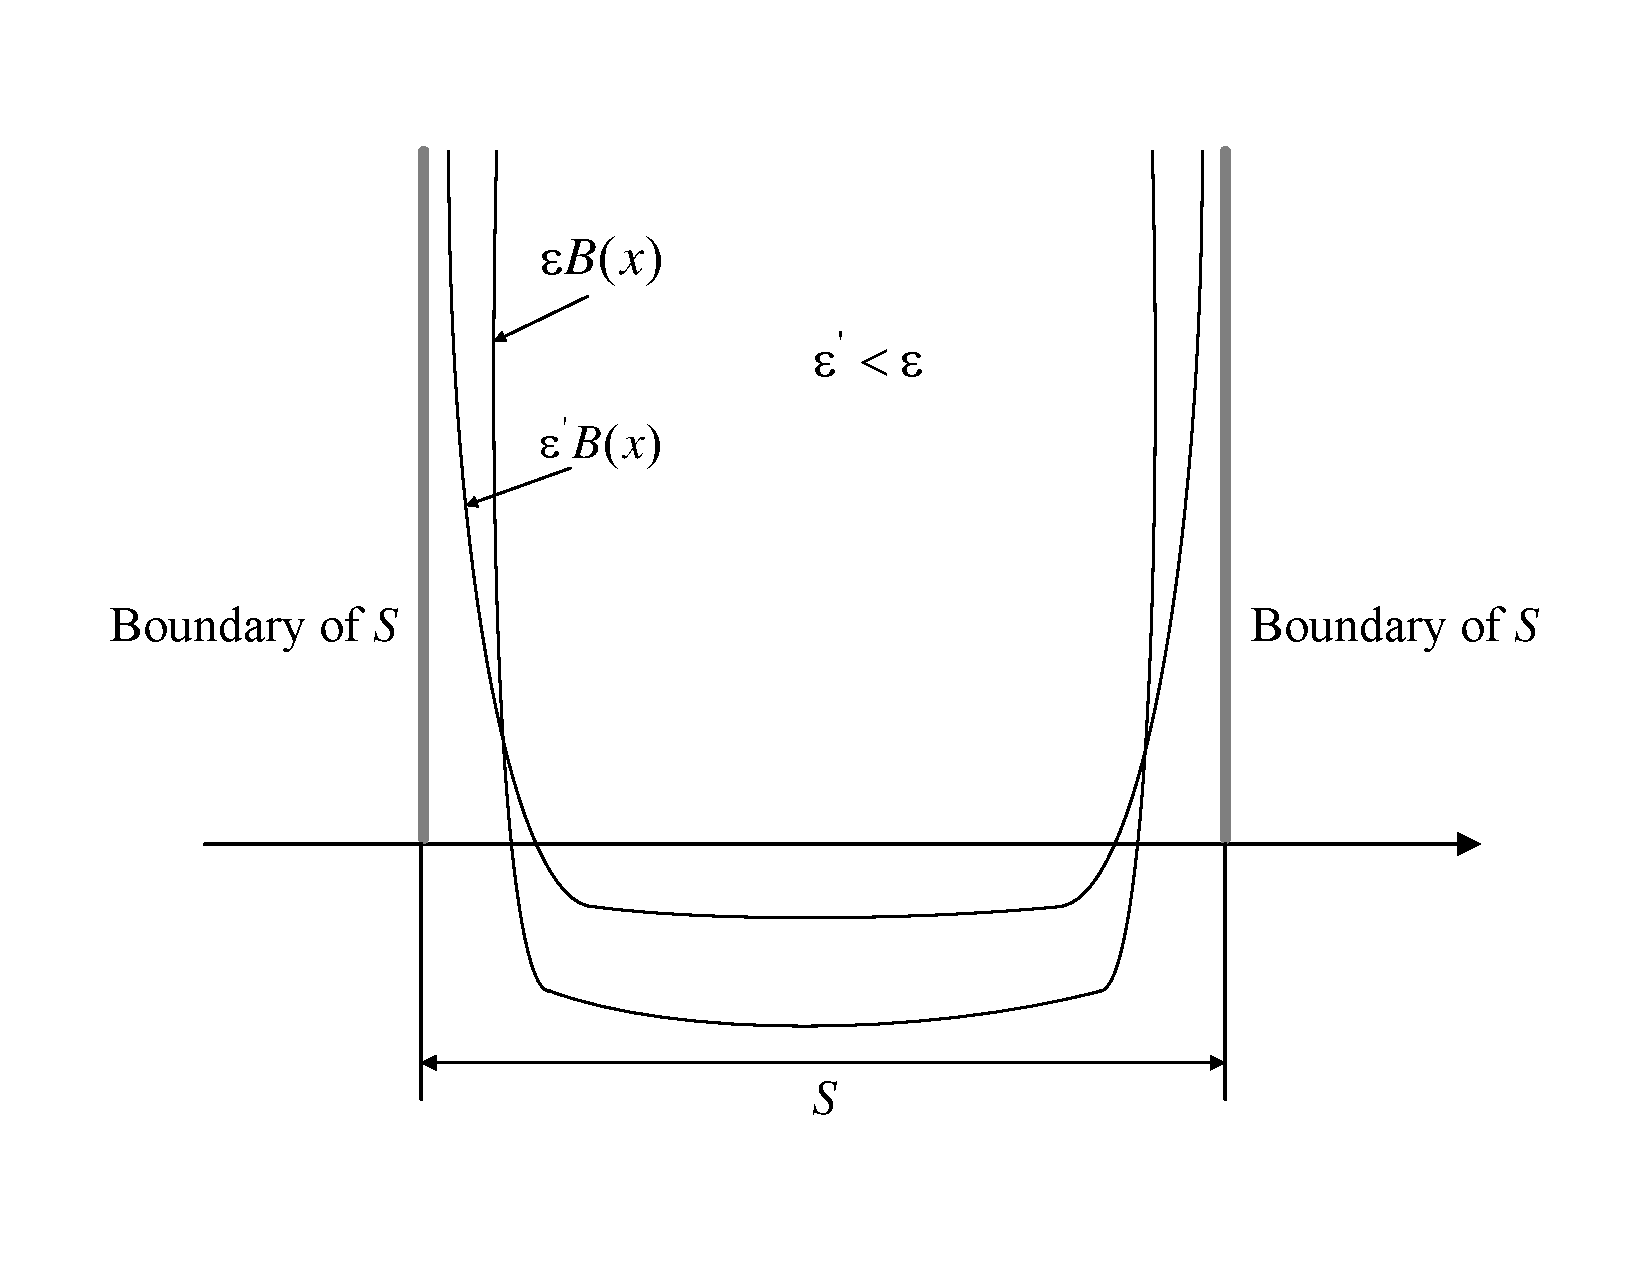
\includegraphics[scale=0.4]{figures/lecture25-barrier_function}
\caption{Form of a barrier term}
\label{fig:barrier}
\end{figure}

Given $B(x)$, define a new cost function $f_\epsilon(x)=f(x)+\epsilon{B(x)}$, where $\epsilon$ is a positive real number. Then we can eliminate the inequality constraints in the original problem and obtain the following problem: 
\begin{equation}
\begin{aligned}
&\min_x & {f_\epsilon(x)}\\
&\qquad\text{s.t.} & x\in{\domain},\\
\end{aligned}
\end{equation}
The form of the barrier term $\epsilon{B(x)}$ is illustrated in Figure \ref{fig:barrier}.

The barrier method is defined by introducing a sequence $\{\epsilon_t\}$ such that $0<\epsilon_{t+1}<\epsilon_t$ for $t=0,1,2,...$ and $\epsilon_t\rightarrow{0}$. Then we find a sequence $\{x_t\}$ such that $x_t\in{\arg \min_{x\in{S}}}f_{\epsilon_t}(x)$. Note that the barrier term $\epsilon_t{B(x)}$ goes to zero for all interior points $x\in{S}$ as $\epsilon_t\rightarrow{0}$, allowing $x_t$ to get increasingly closer to the boundary. Therefore, intuitively, $x_t$ should approach $x^*$ no matter $x^*$ is in the interior or on the boundary of $S$. Its convergence is formalized in the following proposition. 

\begin{proposition}
Every limit point of a sequence $\{x_t\}$ generated by a barrier method is a global minimum of the original constrained problem. 
\end{proposition}
\begin{proof}
See Proposition 5.1.1 of \cite{bertsekas2016nonlinear}.
\end{proof}

As $\domain=\R^n$, Newton's method can be applied with properly selected stepsize to ensure that all iterates lies in $S$. Concretely, an initial interior point can be obtained for some large $\epsilon_0$. Then in each iteration, we can use $x_t$ as an initialization to find $x_{t+1}$ by Newton's method. When $\epsilon_0$ is large, it is easier to find a interior point. And since $x_t$ is close to $x_{t+1}$, it is likely that $x_t$ is in the local convergence region for Newton's method. Therefore, intuitively, global convergence of Newton's method can be enabled by using barrier methods.


\end{definition}
\subsection{Linear Programming}
We'll now adopt the logarithmic barrier method to solve the linear programming (LP) problem defined as follows:
\begin{equation}
\label{eq:LP_def}
\text{LP}:\qquad
\begin{aligned}[c|c|c]
&\min_x &c^T&x\\
&\qquad\text{s.t.} &Ax&\ge b
\end{aligned}
\end{equation}
where $A\in\mathbb{R}^{m\times n}$ with $m\ge n$ and rank($A$)=n. Denote $x^*$ as the optimal point. 

First we write out the augmented cost function by the logarithmic barrier method, i.e.,
\begin{equation}
\label{eq:LP_aug_cost}
f_\epsilon(x) = c^T x-\epsilon \sum_{j=1}^m\ln\left(A^T_j x-b\right).
\end{equation}
where $A^T_j$ is the $j$-th row of $A$. Define $x^*_\epsilon=\argmin_x f_\epsilon(x)$. 

\noindent\textbf{Fact}: $x^*_\epsilon$ exists and is unique for any $\epsilon>0$.
\begin{proof}
We can easily check that $f_\epsilon(x)$ is convex (as a sum of two convex functions). Therefore, the minimizer $x^*_\epsilon$ must exist and is unique.

\textit{Remark}: For the convexity of $f_\epsilon$, we can also check the second-order derivative, which is positive definite as shown in (\ref{eq:hessian_f_eps}) later.
\end{proof}

\subsubsection{Central Path}
The central path of the LP problem in \ref{eq:LP_def} is depicted by the set of $\left\{x^*_\epsilon|\epsilon>0\right\}$, as shown in Fig.~\ref{fig:central_path}.
\begin{figure}[h!]
\centering
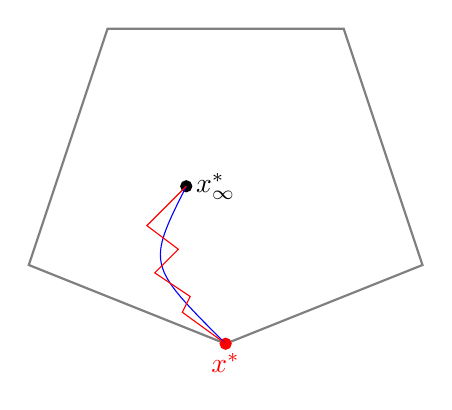
\begin{tikzpicture}
\draw[gray, thick] (-1,2) -- (2,2) -- (3,-1) -- (0.5,-2) -- (-2,-1) -- cycle;
\filldraw[black] (0,0) circle (2pt) node[anchor=west] {$x^*_\infty$};
\filldraw[red] (0.5,-2) circle (2pt) node[anchor=north] {$x^*$};
\draw[blue, thin] (0,0) .. controls (-0.5,-1) .. (0.5,-2);
\draw[red, thin] (0,0) -- (-0.5,-0.5) -- (-0.1,-0.8) -- (-0.4,-1.1) -- (0.05,-1.4) -- (-0.05,-1.6) -- (0.5,-2);
\end{tikzpicture}
\caption{The central path\label{fig:central_path}}
\end{figure}

Our goal is to design an algorithm that will approximately follow the central path. Assume that we already get a "good" enough initial point, then at every step, we apply one step of Newton's method. To guarantee that the algorithm converges, we need to answer the following two questions:
\begin{itemize}
\item Under what conditions that the single-step Newton method works?
\item How to carefully update $\epsilon$?
\end{itemize}

\subsubsection{Newton Decrement}
To apply the Newton's method, first we need to find out the first-order and second-order derivatives of $f_\epsilon$. Note that
\begin{eqnarray}
\triangledown f_\epsilon(x)&=&c-\epsilon \sum_{j=1}^m \dfrac{A_j}{A^T_j x-b}\triangleq c-\epsilon A^T S^{-1}\mathbb{1}\label{eq:grad_f_eps}\\
\triangledown^2f_\epsilon(x)&=&\epsilon A^TS^{-2}A=\epsilon \sum_{j=1}^m\dfrac{A_j A_j^T}{S_j^2}\label{eq:hessian_f_eps}
\end{eqnarray}
where $\mathbb{1}=[1,1,\cdots,1]^T\in\mathbb{R}^{m\times1}$, $S=diag\{A^T_1 x-b, A^T_2 x-b, \cdots, A^T_m x-b\}$.

Then the Newton's update can be applied:
\begin{equation}
\bar{x}=x-[\triangledown^2f_\epsilon(x)]^{-1}\triangledown f_\epsilon(x)=x-[\epsilon A^TS^{-2}A]^{-1}\left(c-\epsilon A^T S^{-1}\mathbb{1}\right)\label{eq:Newton_update}
\end{equation}

Recall that the Newton's method finds the solution by making the first-order condition zero. To measure how much the Newton update will decrease the first-order approximation, we introduce the concept of Newton decrement.

Define the Newton decrement as
\begin{equation}
q^2(x, \epsilon) = \triangledown f^T_\epsilon(x)[\triangledown^2f_\epsilon(x)]^{-1}\triangledown f_\epsilon(x)\label{eq:newton_decrement}
\end{equation}
or $q(x, \epsilon) = [\triangledown^2f_\epsilon(x)]^{-1/2}\triangledown f_\epsilon(x)$. 

Note that the Newton decrement also relates to the difference between $f_\epsilon(x)$ and the minimum of its second-order approximation:
\begin{eqnarray}
&&f_\epsilon(x)-\min_{\bar{x}}\left(f_\epsilon(x)+\triangledown f_\epsilon(x)^T(\bar{x}-x)+(\bar{x}-x)^T\triangledown^2 f_\epsilon(x)(\bar{x}-x)\right)\nonumber\\
&=&f_\epsilon(x)-\left(f_\epsilon(x)-\dfrac{1}{2}\triangledown f^T_\epsilon(x)[\triangledown^2f_\epsilon(x)]^{-1}\triangledown f_\epsilon(x)\right)\nonumber\\
&=&\dfrac{1}{2}\triangledown f^T_\epsilon(x)[\triangledown^2f_\epsilon(x)]^{-1}\triangledown f_\epsilon(x)\triangleq \dfrac{1}{2}q^2(x, \epsilon).
\end{eqnarray}

We now will use the Newton decrement to answer the above two questions: conditions for single-step Newton to work and rules for updating $\epsilon$.

\subsubsection{Propositions, Algorithms and Convergence Theorem}
\begin{proposition}\label{prop1}
Assume $Ax > b$ and $\|q(x, \epsilon)\|<1$, then we have
\begin{align}
c^Tx-c^Tx^{*}\leq 2\epsilon n.
\end{align}
\end{proposition}
In particular, if we maintain that $x_t$ is interior point satisfying $Ax_t>b$,
and $q(x_t, \epsilon_t) < 1$, then $c^{T}x_t$ converges to $c^Tx^*$ as $\epsilon_t$ goes to $0$, i.e., $x_t$ converges to global optimum. However, the condition $q(x_t,\epsilon_t)<1$ is not trivial.  

\begin{proposition}\label{prop2}
If $Ax>b$, and $q(x,\epsilon)<1$, then the pure Newton iterate
step $\bar{x}$ satisfies,
\begin{align}
\|q(\bar{x}, \epsilon)\| &\leq \|q(x, \epsilon)\|^2 
\end{align}
\end{proposition}
It ensures that $\|q(\bar{x}, {\epsilon})\|<1$ given $q(x,\epsilon)<1$ and $x$ is interior point. But we also want that $\|q(\bar{x}, \bar{\epsilon})\|<1$ for some $\bar{\epsilon}<\epsilon$. 

\begin{proposition}\label{prop3}
Assume $q(x,\epsilon)\leq \frac{1}{2}$, interior point $Ax>b$,
put 
\begin{align}
\bar{\epsilon} = (1-\frac{1}{6\sqrt{n}})\epsilon,
\end{align}
then we have
\begin{align}
\|q(\bar{x}, \bar{\epsilon})\|\leq \frac{1}{2}
\end{align}
\end{proposition}
These propositions indicates the following update rule,
\begin{align}
x_{t+1} & = x_t - \nabla^Tf_{\epsilon_t}(x)^{-1}\nabla f_{\epsilon_t}(x_t) \\
\epsilon_t & = (1-\frac{1}{6\sqrt{n}})\epsilon
\end{align}
\begin{theorem}
Suppose $(x_0, \epsilon_0)$ satisfies $Ax_0 >b$ and 
$\|q(x_0,\epsilon_0)\|\leq\frac{1}{2}$, then the algorithm
converges in $\mathcal{O}(\sqrt{n}\log(n/\eta))$ iterations to $\eta$ error, i.e., we have $c^Tx_t\leqslant{c^Tx^*+\eta}$ after $\mathcal{O}(\sqrt{n}\log(n/\eta))$ iterations.
\end{theorem}

\begin{proof}
As Newton step maintains $x_{t+1}$ in the interior, by using the three propositions above, we have 
\begin{eqnarray}
c^Tx_t&\leqslant&{c^Tx^*+2\epsilon_t{n}}\nonumber\\
&=&{c^Tx^*+2(1-\frac{1}{6\sqrt{n}})^t\epsilon_0}\nonumber\\
&\leqslant&{c^Tx^*+2\exp(-\frac{t}{6\sqrt{n}})\epsilon_0}
\end{eqnarray}
Therefore, to have a error of $\eta$, $t\geqslant{\frac{6\sqrt{n}}{\epsilon_0}}\log{\frac{2n}{\eta}}$. We can then conclude that the algorithm converges in  $\mathcal{O}(\sqrt{n}\log(n/\eta))$ iterations to $\eta$ error. 
\end{proof}

The algorithm stated above is the so-called short-step method. Although theoretical convergence rate is guaranteed, the combination of small decrease in $\epsilon$ and a single Newton step is slow in practice. Instead, a more practical method is the so-called long-step method, where $\epsilon$ is reduced in faster rate and several Newton steps are taken per iteration.

\section{List of contributors}

Many thanks to the students of EE227C for their generous help in creating these
lecture notes.

\begin{description}
\item[Lecture 2:] Michael Cheng, Neil Thomas, Morris Yau
\item[Lecture 3:]
\item[Lecture 5:] Victoria Cheng, Kun Qian, Zeshi Zheng
\item[Lecture 6:] Adam Gleave, Andy Deng, Mathilde Badoual
\item[Lecture 7:] Aurelien Bibaut, Zhi Chen, Michael Zhang
\item[Lecture 8:] Eugene Vinitsky
\item[Lecture 11:] Ignasi Clavera, Jianlan Luo
\end{description}

\section{Acknowledgments}

These notes build on an earlier course by Ben Recht, as well as an upcoming
textbook by Recht and Wright. Some chapters also closely follow Bubeck's
monograph on the topic~\cite{Bubeck}.


\bibliographystyle{alpha}
\bibliography{notes}

\end{document}
